%This is the fourth chapter of the dissertation

%The following command starts your chapter. If you want different titles used in your ToC and at the top of the page throughout the chapter, you can specify those values here. Since Columbia doesn't want extra information in the headers and footers, the "Top of Page Title" value won't actually appear.

\pagestyle{cu}
\graphicspath{{./Chapter4/Figures/}}
\chapter[Purity and the Electron Lifetime][Purity and the Electron Lifetime]{Purity and the Electron Lifetime}
\label{chap:purification}

In a noble element dark matter detection experiment the purity of the target mass is an essential consideration and must be measured
continuously.  To date the concentration of electronegative impurities has always been measured in these experiments, but no reliable
model has existed to explain and predict its behavior.

In this chapter I discuss the necessity of extremely pure xenon (\secref{}), explain the original model fit to XENON1T data
(\secref{}), and examine how abrupt changes in detector conditions alter the contamination (\secref{}).



\section{Importance and Procedure for Purifying Xenon}
\secref{sec:importance_procedure}
Purity usually refers to two distinct but correlated values, though the degree of the correlation can depend on the
experiment.  The first is radioactive elements of other noble elements that cannot be completely removed during distillation.  For xenon
our primary challenges are \ce{^{85}Kr} (\secref{subsubsec:backgrounds_electronic_krypton}) and \ce{^{222}Rn}
(\secref{subsubsec:backgrounds_electronic_radon}) as they have low-energy decays that can contaminate our region of interest (while
\ce{^{220}Rn} also leads to a low-energy \betadecay its half-life is too short to penetrate our detector and thus can be ignored).

The second consideration with regards to detector purity is contamination of electronegative impurities such as \ce{O_2} or
\ce{N_2}.  These attach to drifting electrons, lowering or even eliminating the S2.  This can have the largest impact at low energies
since the number of \electron is much fewer.  To correct for the expected initial number of electrons we can use the electron lifetime
$\tau_{\mathrm{e^-}}$, though this must be monitored consistently if not perpetually.  Of course, if the entire cloud of electrons is
removed by these impurities we cannot apply a correction since we have no knowledge of where in the detector it occurred or the energy
deposition.

This chapter is focused on the latter of these two purities, though its examination necessitates consideration of the former as we will
see.



\section{Effects of Electronegative Impurities}
\label{sec:importance_procedure_effects}
Impurities mainly come from outgassing of detector materials and diffusion of elements in the air surrounding the detector through seals,
though for the latter this is primarily limited to noble gases such as \ce{^{222}Rn} (\textbf{check this}).  While many of these
contribute to our electronic recoil background (\secref{subsec:backgrounds_electronic}) they can also decrease the number of photons and
electrons measured.

\subsection{Photon Attenuation}
\label{subsec:importance_procedure_effects_photons}
Contaminants been shown to absorb Xe scintillation (178 nm with ${\sim} 14\ \mathrm{nm}$ spectral FWHM)
(\citeref{Watanabe1953a, Watanabe1953b}).  At concentrations of ppm or higher
the fraction of UV photons that reach the PMTs can be considerably decreased - especially for large detectors.  The intensity due to
photon attenuation is given by

\begin{equation}
I(x) = I_0 e^{-x / \lambda_{\mathrm{att}}}
\end{equation}

\noindent where $I_0$ is initial intensity, $x$ is distance, and $\lambda_{\mathrm{att}}$ is the attenuation length.  It can be written
as $1 / \lambda_{\mathrm{att}} = 1 / \lambda_{\mathrm{abs}} + 1 / \lambda_{\mathrm{scatt}}$ where $\lambda_{\mathrm{abs}}$ and
$\lambda_{\mathrm{scatt}}$ are the the absorption and scatterings lengths, respectively.  For entirely pure xenon
$\lambda_{\mathrm{abs}} \sim \infty$ (\citeref{Baldini2005} found $lambda_{\mathrm{abs}} > 100\ \mathrm{cm}$ at 90\% confidence
level).

The inclusion of impurities, however, can shorten the absorption
length.  \figref{fig:importance_procedure_effects_photons_absorption_coefficents} shows the absorption coefficients
($\lambda_{\mathrm{abs}}^{-1}$) for 1 ppm \htwoo and \otwo from $130 \mdash 200\ \mathrm{nm}$.  They overlap with shorter wavelengths
of the xenon spectrum (included for comparison), meaning measured VUV photons by PMTs will not be symmetric above 178 nm.  With a nearly
1-meter tall detector a 1 ppm concentration of \htwoo would have an effect at 184 nm.

\begin{figure}
\centering
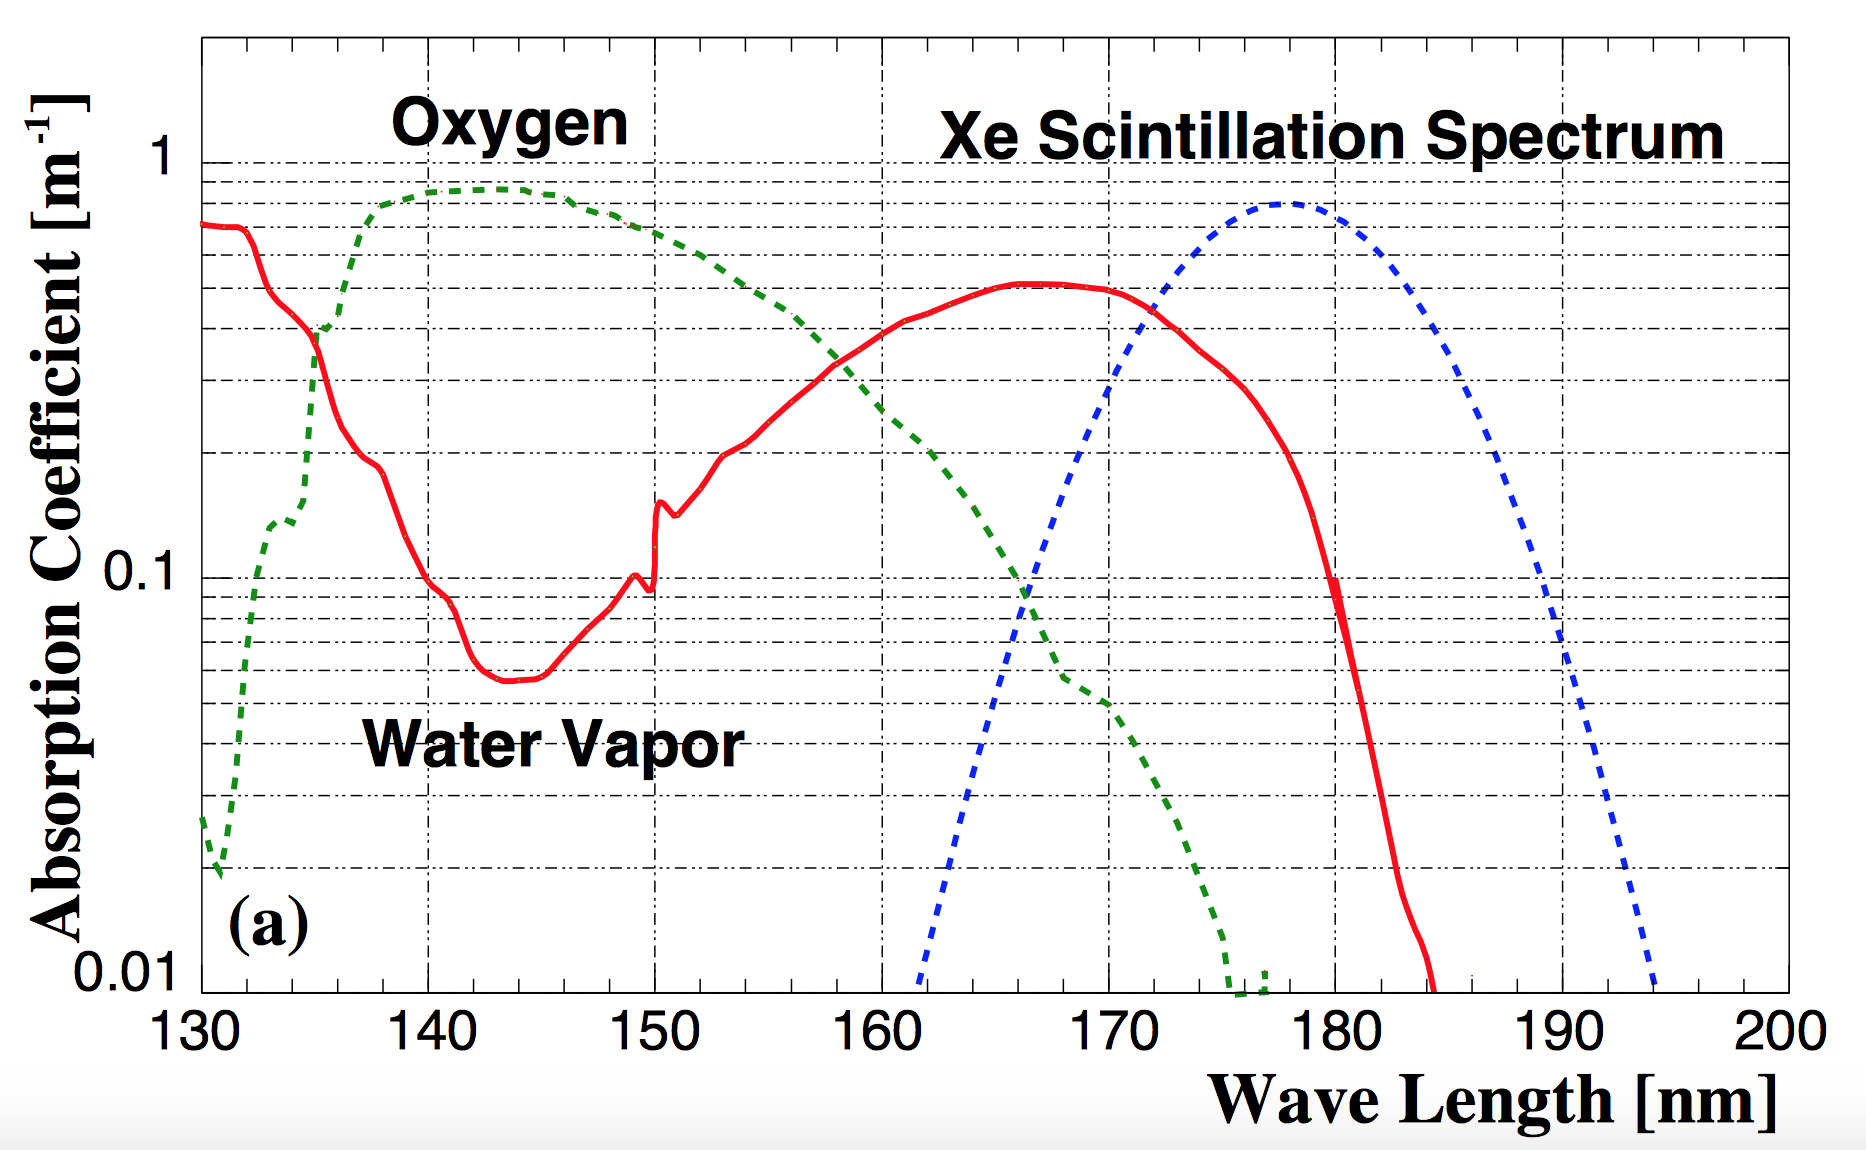
\includegraphics[width=0.8\textwidth]{AbsorptionSpectra}
\caption{Absorption coefficient for photons at 1 ppm \ce{H_2O} vapor (solid red) and \ce{O_2} (dashed green).  The Xe scintillation
spectrum is overlaid for comparison (dashed blue).  \ce{H_2O} impacts Xe scintillation considerably
more than \ce{O_2}.  Image credit: \citeref{Ozone2005}, \ce{H_2O} data from \citeref{Yoshino1996}.}
\label{fig:importance_procedure_effects_photons_absorption_coefficents}
\end{figure}

The relative intensities for different \ce{H_2O}/Xe and \ce{O_2}/Xe concentrations from $0 \mdash 60\ \mathrm{cm}$ are shown in
\figref{fig:importance_procedure_effects_photons_absorption_distance}.  We see that at the level of $\mathcal{O}(100)\ \mathrm{ppb}$ of
oxygen $I / I_0 > 0.8$ at 60 cm.  The effect of water is substantially worse with $I / I_0 < 0.3$, highlighting the necessity of
significant reduction in XENON1T.  Even with a LXe purity that is appreciably better than
\figref{fig:importance_procedure_effects_photons_absorption_distance} $\lambda_{\mathrm{att}} \sim \lambda_{\mathrm{abs}}$ since
the effects of scattering are subdominant with respect to absorption.

\begin{figure}
\centering
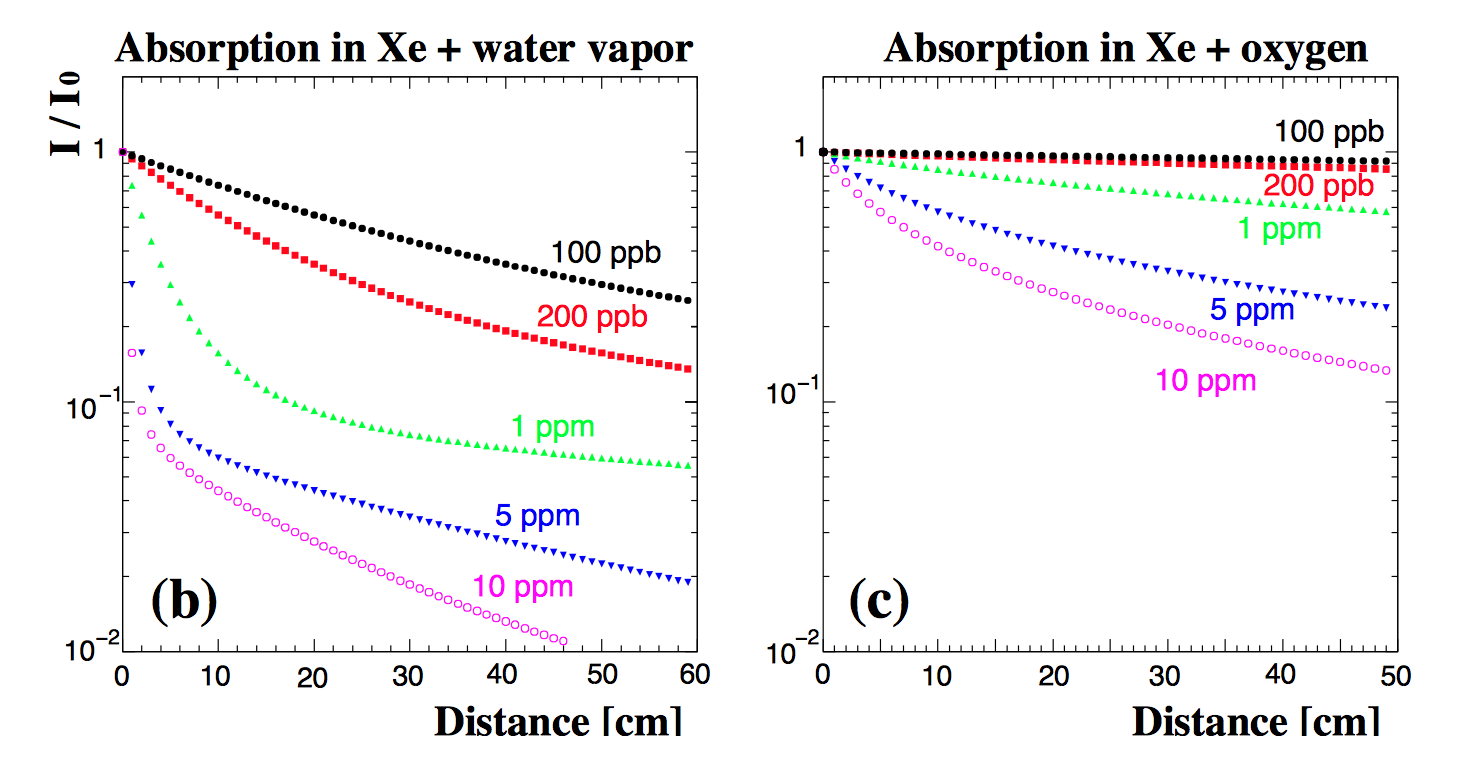
\includegraphics[width=\textwidth]{AbsorptionWithDistance}
\caption{Fraction of initial intensity of xenon scintillation with distance for various concentrations of \htwoo (left) and \otwo
(right).  Image credit: \citeref{Ozone2005}.}
\label{fig:importance_procedure_effects_photons_absorption_distance}
\end{figure}

Photon attenuation ultimately increases our energy threshold as we are less sensitive to lower energies as few photons are
measured.



\subsubsection{Charge Depletion}
\label{subsubsec:importance_procedure_effects_charge}
Electrons that do not recombine will drift antiparallel to $E_d$ in an electron cloud.  As the electron cloud drifts it diffuses both
longitudinally (in the direction of $E_{d}$) and transversely (perpendicular to $E_{d}$).  The
diffusion coefficients $D_{L}$ and $D_{T}$ are dependent on the electric field with $D_{T}/D_{L} \sim 10$.  The electron spread can
be written as $\sigma_{D_{T}} = \sqrt{D_{T} t_{d}}$ where $t_{d} = d/v_{d}$ is the drift time and $d$ is the drift distance.

The behavior of electrons can be classified according to their mobility in the limit of $E \rightarrow 0$, $\mu_0$.  When LXe is
polarized by electrons its high polarizability ($4.0 \times 10^{-24}\ \mathrm{cm^3}$, highest for noble gas) will both make it
attractive to \electron and interact with nearby Xe atoms through dipole-dipole interaction.  The equilibrium of these two effects
determines the potential energy of the ground state of electrons $V_0$, which is anti-correlated with $\mu_0$.  For LXe these have
been measured to be $V_0 = -0.61 \pm 0.05\ \mathrm{K}$ (\citeref{Tauchert1977}) and $\mu_0 = 2200 \pm 200\ \mathrm{cm^2\ V^{-1}\ s^{-1}}$
(\citeref{Yoshino1976}) at $165\ \mathrm{K}$ (in addition $\mu_0$ was found to be $1900$ and $2200\ \mathrm{cm^2\ V^{-1}\ s^{-1}}$
at $163\mathrm{K}$ by \citeref{Yoshino1976} and \citeref{Miller1968}, respectively).  The large electron mobilities indicate the
electrons are \textit{quasifree}, and have drift velocities that can exceed even those of GXe, as shown in
\figref{fig:importance_procedure_effects_charge_drift_velocity}.

\begin{figure}
\centering
\includegraphics[width=0.8\textwidth]{drift_velocity_field}
\caption{Drift velocity (defined as $W$ here) dependence on reduced electric field $E/N$ where $N$ is the number of molecules per
volume.  Points are from experimental data (\citeref{Gushchin1982, Huang1978, Wagner1967, Pack1992}) and curves are from
calculations.  $1\ \mathrm{Td} = 10^-17\ \mathrm{V\ cm^2}$.  LXe has a higher drift velocity than GXe at
$E/N \lesssim 1\ \mathrm{Td}\ (1\ \mathrm{Td} = 10^{-17}\ \mathrm{V\ cm^2})$.  Image credit: \citeref{Atrazhev2005}.}
\label{fig:importance_procedure_effects_charge_drift_velocity}
\end{figure}

Ions exhibit significantly lower mobility than electrons.  It is parameterized as $\mu \approx \eta^{-\alpha}$ where $\eta$ is the
liquid viscosity and $\alpha = 1 \mdash 2$.  The diffusion coefficients can be calculated with the Nernst-Einstein equation

\begin{equation}
\frac{e D(E)}{\mu (E)} = \mathcal{F} <E>
\end{equation}

\noindent where $\mathcal{F} = 0.5 \mdash 1$ is depends on the electron distribution function (e.g. $\mathcal{F} = 2/3$ for a
Maxwellian distribution).

The mobilities for holes, \ce{TMSi^+}, \ce{O_2^-}, \ce{^{226}Th}, \ce{^{208}Tl}, and \ce{Xe_2^+} in in LXe are listed in
\tabref{tab:importance_procedure_effects_charge_mobilities}.  They are ${\sim} 10^6$ times smaller than the electron mobility.

\begin{table}
\centering
\begin{tabular}{cccccc}
Ion & T [K] & $\mu\ [10^{-4}\ \mathrm{cm^2\ V^{-1}\ s^{-1}}]$ & Ref. \\
\hline
holes & 161 & 35 & \citeref{Hilt1994b} \\
holes & 230 & 46 & \citeref{Hilt1994b} \\
\ce{TMSi^+} & 162 & 2 & \citeref{Hilt1994a} \\
\ce{TMSi^+} & 192 & 3 & \citeref{Hilt1994a} \\
\ce{O_2^-} & 162 & 6 & \citeref{Hilt1994a} \\
\ce{O_2^-} & 192 & 10 & \citeref{Hilt1994a} \\
\ce{^{226}Th^+} & 162 & 2.4 & \citeref{Wamba2005} \\
\ce{^{208}Tl^+} & 163 & 1.33 & \citeref{Walters2003} \\
\ce{Xe_2^+} & 184.2 & 2.85 & \citeref{Davis1962} \\
\ce{Xe_2^+} & 192.1 & 3.17 & \citeref{Davis1962} \\
\hline
\end{tabular}
\caption{Ion mobilities in LXe.  All ions listed are positive with the exception of \ce{O_2^-}.  Positive holes have mobilities that are
${\sim} 10$ greater than ions.  Summarized data is given in \citeref{Aprile2006a}.}
\label{tab:importance_procedure_effects_charge_mobilities}
\end{table}

Hole mobility can be described by the hopping model of charge carrier transport.  In this temperature-dependent model charge is
propagated through jumps between traps yielding

\begin{equation}
\mu = \frac{e b^2}{k_{\mathrm{B}} T} \omega
\label{eq:importance_procedure_effects_charge_mobility_simple}
\end{equation}

\noindent where $b$ is the average jump distance and $\omega$ is the jumping frequency, parameterized as

\begin{equation}
\omega = P \Big( \frac{\omega_0}{2 \pi} \Big) e^{-E_{\mathrm{a}} / k_{\mathrm{B}} T}
\end{equation}

\noindent where $\omega_0$ is the phonon frequency, $P(\omega_0 / 2 \pi)$ is the tunneling probability between adjacent holes with
activation energy $E_{\mathrm{a}}$.  \figref{importance_procedure_effects_charge_hole_mobility} shows hole mobility in
LXe.  The solid curve represents a model that parameterizes \eqref{eq:importance_procedure_effects_charge_mobility_simple} as

\begin{equation}
b^3(T) = \sqrt{2} M / \rho (T)
\end{equation}

\noindent where $M$ is the atomic mass of xenon and $\rho (T)$ is the temperature-dependent density (\citeref{Hilt1994b}).  It
additionally assumes the hole is self-trapped between two rare atoms in a potential well, forming a polaron.  It gives a hole mobility of

\begin{equation}
\mu (T) = \frac{e b^2 (T)}{k_{\mathrm{B}}} \frac{2 \pi}{h} \sqrt{\frac{\pi}{4 E_a k_{\mathrm{B}} T}} J_0^2
e^{-2 \alpha b(T)} e^{-E_a / k_{\mathrm{B}} T}
\label{eq:importance_procedure_effects_charge_mobility_polaron}
\end{equation}

\noindent where $h$ is Planck's constant and and $J(T) = J_0 e^{-\alpha b(t)}$ is the transfer integral.

\begin{figure}
\centering
\includegraphics[width=0.8\textwidth]{hole_mobility}
\caption{Fig. 3.15 in Aprile book.  Temperature-dependent drift mobility for holes in LXe.  Data is shown as empty triangles.  A fit
using \eqref{eq:importance_procedure_effects_charge_mobility_polaron} is shown as the solid line.  Image credit: \citeref{Aprile2006a}
(redrawn from \citeref{Hilt1994b}.)}
\label{fig:importance_procedure_effects_charge_hole_mobility}
\end{figure}

As the cloud drifts electronegative impurities can bond to \electron and prevent them from reaching the liquid-gas interface, thereby
decreasing proportional scintillation

\begin{equation}
e^{-} + S \rightarrow S^{-}
\label{eq:impurity_attach}
\end{equation}

\noindent where $S$ refers to the impurity (e.g. $e^- + \mathrm{O_2} \rightarrow \mathrm{O_2^-}$).

\begin{enumerate}
\item Radiative attachment is given by
\begin{equation}
e^- + XY \rightarrow XY^- + h \nu
\end{equation}

\noindent where $XY$ is some atom or molecule.

\item Dissociative electron attachment (DEA) is when a low-energy electron bonds to a molecule causing it to fracture.  The process
is given by

\begin{equation}
\begin{aligned}
e^- + XY \rightarrow XY^* + e^- \rightarrow X^+ + Y^- + e^- \\
e^- + XY \rightarrow XY^- \rightarrow X + Y^-
\end{aligned}
\end{equation}

\noindent where molecule $XY$ is separated into components $X$ and $Y$.  \ce{O_2} has 5.116 eV dissociation energy and \ce{O^-} has
electron affinity of 1.461 eV.

\item Three-body attachment proceeds via the two-stage Bloch-Bradbury reaction (\citeref{Bloch1935, Herzenberg1969})

\begin{equation}
\begin{aligned}
e^- + XY &\leftrightarrow (XY^-)* \\
(XY^-)^* + Z &\rightarrow XY^- + Z
\end{aligned}
\end{equation}

\noindent where $Z$ is an atom or molecule from the majority gas population.  It carries out the bonding energy between the
\electron and electronegative $XY$.  Oxygen was studied (\citeref{Aleksandrov1993, Aleksandrov1981, Aleksandrov2009}).
\end{enumerate}



\section{Electron Lifetimes}
\label{sec:electron_lifetimes}
Nearly any mono-energetic radioactive decay can be used to measure the electron lifetime.  For XENON1T electron lifetimes were calculated
using the elements listed in \tabref{tab:electron_lifetimes_isotopes}.  An additional method of minimizing the \stwob band width using the
\ce{^{212}Pb} electronic recoil band to address an emerging discrepancy between
$\mathrm{^{83m}Kr}$ and \alphadecays (\secref{subsec:electron_lifetimes_rn222_vs_kr83m}) was tried but had too large of an uncertainty
to render itself valuable.

Following an \ambe or neutron generator calibration $\mathrm{^{129}Xe}$ and $\mathrm{^{131}Xe}$ will be in excited nuclear states
(\secref{subsubsec:electron_lifetimes_measurement_gammas}).  Their
$\gamma$-emissions and uniform distribution in the TPC make them excellent candidates to measure the electron lifetime for electronic
recoils.  Unfortunately their half-lifes of 8.88 and 11.93 d, respectively, eliminate any statistically significant results after more
than a few weeks.

\begin{table}
\centering
\begin{tabular}{rccrcc}
\hline
\hline
Isotope & Decay & Energy & $t_{1/2}$ & Section & Notes \\
\hline
$\mathrm{^{83m}Kr}$ & $\beta^-$ & $32.2\ \mathrm{keV}$ & 1.83 h & \secref{subsec:electron_lifetimes_measurement_kr} & Calibration \\
$\mathrm{^{129m}Xe}$ & $\gamma$ & $236.2\ \mathrm{keV}$ & 8.88 d & \secref{subsec:electron_lifetimes_measurement_gammas} & Background following NR cal. \\
$\mathrm{^{131m}Xe}$ & $\gamma$ & $163.9\ \mathrm{keV}$ & 11.93 d & \secref{subsec:electron_lifetimes_measurement_gammas} & Background following NR cal. \\
\ce{^{212}Bi} & $\alpha$ & $6.207\ \mathrm{MeV}$ & 60.55 m & \secref{subsec:electron_lifetimes_measurement_alphas} & \ce{^{220}Rn} calibration \\
\ce{^{218}Po} & $\alpha$ & $6.115\ \mathrm{MeV}$ & 3.10 m & \secref{subsec:electron_lifetimes_measurement_alphas} & Background \\
\ce{^{222}Rn} & $\alpha$ & $5.590\ \mathrm{MeV}$ & 3.82 d & \secref{subsec:electron_lifetimes_measurement_alphas} & Background \\
\hline
\hline
\end{tabular}
\caption{Isotopes used for electron lifetime analysis.  Background \ce{^{222}Rn} and \ce{^{218}Po} \alphadecays allowed continual
monitoring of but had relatively low statistics.  $\mathrm{^{83m}Kr}$ and \ce{^{212}Bi} had high statistics but were only available during
calibrations.  Excited nuclear states $\mathrm{^{131m}Xe}$ and $\mathrm{^{129m}Xe}$ were present in background after nuclear recoil
calibrations but their half-lifes decreased viability after several weeks.}
\label{tab:electron_lifetimes_isotopes}
\end{table}



\subsection{Measuring the Electron Lifetime}
\label{subsec:electron_lifetimes_measurement}
The electron lifetimes over the XENON1T lifetime is shown in \figref{fig:electron_lifetimes_evolution_no_model}.  Initially lifetimes were
measured by selecting single-scatter data.



\subsubsection{S2/S1}
\label{subsubsec:electron_lifetimes_measurement_ss}
In the period immediately following XENON1T becoming operational the electron lifetime was ${\sim} 0$ since purification began at roughly
the same time.  The first in-situ calibration would not be performed until almost three months later and using any mono-energetic
background decays (which had not yet been investigated) would have given too few events in the top of the detector to be reliable.

Without being able to isolate any mono-energetic events S2 alone would be unable to establish the electron lifetime.  However,
S2/S1 - while not truly energy-independent - was enough so to give a reasonable estimate.  It was too early to have official cuts but
the ones used were sufficient and based on a history of knowledge of TPC detectors.

S1 (S2) single scatter cuts required that the second largest S1 (S2) be $< 0.2$ that of the first.  The purpose of these cuts was to
prevent S1-S2 mismatching: the S1 cut would
remove the possibility that we do not observe the S2 of a scatter deep in the TPC, while the S2 eliminated ambiguity in matching a single
S1 with two potential S2s.

To reject noise at least three PMTs must observe the S1.  This is the same cut that was used in the dark matter analysis.  Finally, the
fraction of light seen on the top PMT array must fall between $0.2 \mdash 0.6$ for S1s and $0.5 \mdash 0.9$ for S2s.

On a few occasions a \ce{^{137}Cs} was placed outside the detector.  While the LXe self-shielding limited the fraction of radiation that
made it inside the TPC enough events were present to get a dependable value.  This method was used until early August 2016.



\subsection{$\alpha$-Decays}
\label{subsec:electron_lifetimes_measurement_alphas}
The high energy and substantial stopping power (\figref{fig:mass_stopping_power}) of $\alpha$ interactions creates significant
recombination, in turn creating an S1 that makes them easily distinguishable from electronic and nuclear
interactions.  Because they are easily recognizable and do not scatter many of the cuts developed for the science run analysis are not
necessary (many are in addition not reliable since they were developed using low-energy electronic recoils).  There are just a small
number of cuts that are used.

Events must have $r_{\mathrm{rec}} < 36.94\ \mathrm{cm}$.  This is in part for consistency with the First Results FV
(\citeref{Aprile2017f}).  But we can also expect inhomogeneity in the electric field to be greatest near the top, bottom, and sides of the
TPC as seen in \figref{fig:xenon1t_tpc_efield}.  Changes in the field would produce different light and charge yields
(\secref{subsec:det_char_ly_cy}), so the number $\gamma$s and escaped \electron would vary according to position.  Because $\alpha$
LY and QY have little dependence on field this effect is likely to be small or negligible.  However, a more alarming effect is impurity
attachment rate dependence on field, discussed in \secref{subsec:electron_lifetime_model_field}.  Finally, the radial cut removes any
chance of \alphadecays near the wall that would lose drifting \electron to the PTFE.

The fraction of light seen by the top PMTs from electroluminescence is tightly constrained due to the extraction occurring above the
liquid and over the roughly the same distance.  The percentage of events that fail this cut is small but it is important to remove any
``fake'' or gas-events (a cut on the S1 fraction seen by the top PMTs will also distinguish GXe events).

In addition data acquisition quality cuts are used in data selection.  The first is the high energy veto, which is triggered by a very
large S2.  The second is produced by one or more digitizers nearly filling its memory buffer, and is called a busy veto.  The third is
a busy type check, which removes events that have a busy signal anywhere in the waveform.  The final is an end of run check, which
disqualifies the last 21 per run (each run is 1 hour).  Details on each are given in \secref{subsec:xenon1t_daq}.

\figref{fig:electron_lifetimes_measurement_alphas_s1} shows cS1 dependence on $z$ for \alphadecays of \ce{^{222}Rn}
(${\sim} 5.1 \times 10^4 \ \mathrm{PE}$) and \ce{^{218}Po} (${\sim} 5.6 \times 10^4\ \mathrm{PE}$) after these cuts.  The large
S1s from events deep in the detector can saturate PMTs in the bottom array, which lead to under-corrected cS1s as seen in the left
panel.  To correct for this the data are split into slices in $z$ and fit in cS1 with gaussians.  Fits in the region
$-40 \lesssim z \lesssim -10 \mathrm{cm}$ where saturation is not present are interpolated to build a cS1 distribution, which is
extrapolated across the entire length of
the TPC.  Differences in fit parameters are used to relocate events deeper in the detector into the proper cS1 band.  The
$\alpha$-corrected cS1 distribution is shown in the right panel of \figref{fig:electron_lifetimes_measurement_alphas_s1}.

\begin{figure}
\centering
\includegraphics[width=\textwidth]{rn_po_cs1_alpha}
\caption{cS1 (left) and $\alpha$-corrected cS1 (right) dependence on $z$.  The large \alphadecay S1s deep in
the TPC sature the bottom PMTs causing an under-corrected cS1, which
results in the distortion seen in the left panel.  Near the top ($z \lesssim -10\ \mathrm{cm}$) a similar effect is observed from top PMT
saturation.  The distortion is corrected in the right panel where the effect is much less significant.  The red and blue boxes highlight
the events selected to calculate $\tau_e$.  The colors of data markers correspond to \stwob values.}
\label{fig:electron_lifetimes_measurement_alphas_s1}
\end{figure}

Even with the $\alpha$-corrected cS1s we can still see there is saturation near the very bottom of the TPC.  The saturation is so great
here that events from \ce{^{222}Rn} and \ce{^{218}Po} cannot be distinguished from one another.  This is generally not a problem since it
is outside our fiducial volume.  There is also some distortion at $z \gtrsim$ from events
near the LXe surface, whose light is tightly concentrated in the top PMT array.

The selected \ce{^{222}Rn} and \ce{^{218}Pb} events are indicated by color and color boxes, respectively.  Events with
$-89< z < -9\ \mathrm{cm}$ and
$4.9 \times 10^4 < \alpha \mdash \mathrm{corrected\ cS1} < 5.3 \times 10^4\ \mathrm{PE}$ (\ce{^{222}Rn}) and
$5.35 \times 10^4 < \alpha \mdash \mathrm{corrected\ cS1} < 5.8 \times 10^4\ \mathrm{PE}$ (\ce{^{218}Po}) are selected.  The electron
lifetime is calculated for each
independent of the other, which provides a nice cross-check.  Because \ce{^{218}Po} has a half-life of just 3.1 m the number of events
should be roughly the same.  Each electron lifetime is calculated from 48 hours of data to get sufficient statistics.

The data is binned in $\delta t_d$ and an initial fit is performed on the 50th percentiles of the \stwob distributions from each
slice.  This preliminary electron lifetime $\tau_e^{(\mathrm{p})}$ is used to remove events that are far from the distribution.  The data
is then additionally binned in cS1 and fit with a gaussian in each $\delta t_d$ slice.  The means and standard deviations are then fit
with an exponential, yielding the final electron lifetime $\tau_e$.  An example can be seen in
\figref{fig:electron_lifetimes_measurement_alphas_elifetime}.  The color (color) dashed lines define the boundaries above (below) which
events were cut with the preliminary fit.  Both fits are plotted in each panel for comparison.  We can see \ce{^{222}Rn} (left) and
\ce{^{218}Po} (right) give good agreement.

\begin{figure}
\centering
\includegraphics[width=\textwidth]{rn_po_electron_lifetime_log}
\caption{Electron lifetime measurements using \ce{^{222}Rn} (left) and \ce{^{218}Po} (right) from October 29-31, 2017.  The red and blue
lines correspond to \ce{^{222}Rn} and \ce{^{218}Po}, respectively, and are drawn in the drift time region that was used for the fit (see
text for event selection).  They are each shown in both panels to show the \stwob overlap, highlighting the need for the
$\alpha$-corrected cS1 cut.  The pink dashed lines mark the boundaries derived from the preliminary fit outside of which events were not
considered in the final fit.  The electron lifetime measurements agree within uncertainty.}
\label{fig:electron_lifetimes_measurement_alphas_elifetime}
\end{figure}

The overlap in \stwob highlights the necessity of using cS1 as a selection criterion.  Originally a cS1 $\alpha$-correction map did not
exist so \ce{^{222}Rn} and \ce{^{218}Po} were fit together.  This turned out to yield slightly lower $\tau_e$ than separate fits.  Once
the $\alpha$-correction was lifetimes was re-computed; however, this was not possible for some of the earlier data that had been
deleted.

This method can in principle be achieved for any $\alpha$-emitting element distributed throughout the FV of the detector and is done so
for \ce{^{212}Bi} during \ce{^{220}Rn} calibrations.


\subsection{$\mathbf{^{83m}Kr}$}
\label{subsec:electron_lifetimes_measurement_kr}
The delayed coincidence between the 32.2 and 9.4 keV decays help differentiate $\mathrm{^{83m}Kr}$ events from background.  With
$t_{1/2} = 154\ \mathrm{ns}$ for the 9.4 keV a large fraction of the S1s will overlap so a cut
$600 < \delta t_{\mathrm{S1}} < 2000\ \mathrm{ns}$
where $\delta t_{\mathrm{S1}}$ is the time between S1s is applied.  In addition we require the number of PMTs that see the 9.4 keV peak
to be $> 3$ to avoid coincident PMT noise and $< 30$ since it is low-energy.

The electron lifetime is calculated using the 32.2 keV decay with a procedure similar to that described in
\secref{subsubsec:electron_lifetimes_measurement_alphas}.  An preliminary fit is performed using the median \stwob in each drift time
slice.  However, the high statistics and near-total background removal by the $\delta t_{\mathrm{S1}}$ cut
removes the need to exclude events far from the true \metakr.  Next each $\delta t_d$ slice is fit with a gaussian and an exponential
is then fit to the the results.



\subsection{$\mathbf{\gamma}$-rays}
\label{subsec:electron_lifetimes_measurement_gammas}
The full absorption peak of \gammarays make them great candidates for electron lifetime measurements.  Unfortunately nearly all
\gammarays in the TPC come from elements in detector materials or external sources placed inside the water tank
(e.g. \ce{^{137}Cs}).  However, nuclear recoils can excite \ce{^{129}Xe} and \ce{^{131}Xe} nuclei with half-lifes
of 8.88 and 11.93 days, respectively.  These metastable states serve as an in-situ calibration that can be used to measure a number of
detector parameters including light and charge yield (\secref{subsec:det_char_ly_cy}), $g_1/g_{2\mathrm{b}}$
(\secref{subsec:det_char_photon_charge_efficiencies}), and electron lifetime.  While these evaluations can validate fellow
electronic recoil measurements from \meta{83m}{Kr}, the short $t_{1/2}$ limit these to the few weeks following an \ambe or NG
calibration due.

Selecting \meta{129}{Xe} and \meta{131}{Xe} events is trickier than $\alpha$ or \meta{83}{Kr}.  This is in part because they sit
on top of an ER background (see \figref{fig:calibrations_photon_charge_efficiences_ces_resolution} for background energy spectrum), have a
relatively low event rate, and do not have properties that allow a high-percentage cut
efficiency (e.g. \meta{83}{Kr} delayed coincidence).  Instead a number of cuts need to be applied to remove unwanted data before a fit
can be done.

To select the 163.9 and 236.2 keV peaks an S2 single scatter cut is used to remove the underlying background.  Additional data quality
cuts include ensuring the fraction of the S2 seen by the top PMTs and the width of the S2 fall within known distributions.  For the FV
we apply the usual $r_{\mathrm{rec}} < 36.94\ \mathrm{cm}$ but require $-85 < z < -10\ \mathrm{cm}$ to remove \gammarays on the same
energy scale from surrounding materials that can penetrate deeper into the detector.

Because cS1 is known fitting the $\gamma$ peaks is reasonably simple, especially if the electron lifetime can be roughly estimated.  In
\figref{fig:electron_lifetimes_measurement_gammas_s1_s2} they are shown surrounded by contours from two-dimension gaussian fits.  The
y-axis is labeled as \cstwob because for this data $tau_e$ is known within small uncertainty - however, generally speaking this is not
the case.  The final cut we use then is to remove data outside some $\sigma$.

\begin{figure}
%    \centering
    \begin{subfigure}[t]{0.4\textwidth}
%        \centering
        \includegraphics[height=4cm]{}
    \end{subfigure}%
    \begin{subfigure}[t]{0.65\textwidth}
%        \centering
        \includegraphics[height=4cm]{}
    \end{subfigure}
    \caption{}
	\label{fig:electron_lifetimes_measurement_gammas_s1_s2}
\end{figure}

To verify the data we've selected is primarily \meta{129}{Xe} and \meta{131}{Xe} the event rate can be fit as seen in
\figref{fig:electron_lifetimes_measurement_gammas_decay_rate} shows the number of decays in the two months following the
SR0 \ambe calibration.  The fits give half-lifes that agree with the true values.  A constant is included to account for underlying
background.

\begin{figure}
\centering
\includegraphics[width=\textwidth]{xe_meta_decay_rate}
\caption{$\mathrm{^{129m}Xe}$ and $\mathrm{^{131m}Xe}$ events following the SR0 \ambe calibration.  Data is omitted during \metakr
and \ce{^{220}Rn} calibrations.  Fits using $R(t) = R_0 \mathrm{exp}(-t/t_{1/2}) + C$ give half-lifes of $8.66 \pm 0.26$ and
$11.51 \pm 0.43$ days, respectively, which match the known rates of 8.88 and 11.93 days.}
\label{fig:electron_lifetimes_measurement_gammas_decay_rate}
\end{figure}

The procedure to calculate $\tau_e$ is the same as in \secref{subsubsec:electron_lifetimes_measurement_alphas}.  The result for the
$num$ days following the \ambe calibration in \figref{fig:electron_lifetimes_measurement_gammas_decay_rate} (dateone to datetwo)
is shown in \figref{fig:electron_lifetimes_measurement_gammas_elifetime}.

\begin{figure}
\centering
\includegraphics[width=\textwidth]{}
\caption{Electron lifetimes using \meta{129}{Xe} and \meta{131}{Xe} 236.2 and 163.9 keV $\gamma$-rays.}
\label{fig:electron_lifetimes_measurement_gammas_elifetime}
\end{figure}

\begin{figure}
\centering
\includegraphics[width=\textwidth]{electron_lifetime_evolution_no_model}
\caption{Electron lifetimes of \ce{^{222}Rn} (yellow triangles), \ce{^{220}Rn} (red triangles), \ce{^{218}Po} (turquoise triangles), and
\metakr (green circles) over the
XENON1T experiment.  We can see the lifetimes computed from \alphadecays differ from those of \metakr.}
\label{fig:electron_lifetimes_evolution_no_model}
\end{figure}



\subsection{\ce{^{222}Rn} vs. $\mathbf{^{83m}Kr}$}
\label{subsec:electron_lifetimes_rn222_vs_kr83m}
\figref{fig:electron_lifetimes_evolution_no_model} shows clear disagreement of electron lifetimes between $\alpha$-emitters and \metakr
at $\tau_e \gtrsim 400\ \mathrm{\mu s}$.  This presents a challenge for correcting \stwob for signals in the TPC.

The discrepancy is the result of field non-uniformity in the TPC (\figref{fig:xenon1t_tpc_efield}).  Because the change in recombination
of \alphadecays differs from that of electronic recoils (\figref{fig:tpcs_signals_drift_field}) the ratio of the \electron yields vary
inhomogeneously across the detector.  Thus two issues are apparent.  The first is bias will be present between any two events of equal
energy and type that occur at different fields in the detector.  Therefore we expect \metakr, $\mathrm{^{129m}Xe}$, and
$\mathrm{^{131m}Xe}$ to not accurately report the xenon purity.  The second is two events whose \electron yield changes in electric field
$dE/de^-$ are dissimilar require independent lifetime corrections.  LUX also observed a disparity between \metakr and \ce{^{222}Rn}
lifetimes as well as field inhomogeneity (\citeref{LUX2017d, Knoche2016}).

In \figref{fig:electron_lifetimes_rn222_vs_kr83m_field_tpc} the electron yields for $\mathrm{^{129m}Xe}$ and \ce{^{222}Rn}
are shown throughout the TPC according to NEST (\citeref{NEST2013}). (assuming azimuthal symmetry).  The yields are normalized to the
region [$-90 \leq z \leq -85\ \mathrm{cm}$,
$r < 36.94\ \mathrm{cm}$].  The 1-ton fiducial volume is marked by the black line.  Both have decreasing yields in the $-z$ direction,
with the deviation for \ce{^{222}Rn} being more than twice as large as $\mathrm{^{129m}Xe}$.  This means $\tau_e$ is biased towards
smaller values but the effect is more significant for \ce{^{222}Rn} and other $\alpha$-decays.

S1 below 10 keV has minimal field dependence because recombination is minimal.  Over 10 keV recombination increases.

\begin{figure}
\centering
\includegraphics[width=\textwidth]{relative_electron_yield_field_tpc}
\caption{Relative \electron yield with respect to [$-90 \leq z \leq -85\ \mathrm{cm}$, $r \geq 36.94\ \mathrm{cm}$] for
$\mathrm{^{129m}Xe}$ (left) and \ce{^{222}Rn} (right) for ${\sim}120\ \mathrm{V\ cm^{-1}}$ inside the 1T FV (black line).  A decline in
yield is
observed moving in the $-z$ direction, which leads to a misleading observation that the electron lifetime is lower than its true
value.  The imbalance between the top
and bottom of the TPC is $\gtrsim 2\times$ larger for \ce{^{222}Rn}, causing it to appear lower than its $\gamma$ counterparts.}
\label{fig:electron_lifetimes_rn222_vs_kr83m_field_tpc}
\end{figure}

The $z$-dependence of \electron yields for $\mathrm{^{129m}Xe}$, $\mathrm{^{131m}Xe}$, \ce{^{60}Co}, \ce{^{208}Tl}, and \ce{^{222}Rn} is
plotted in \figref{fig:electron_lifetimes_rn222_vs_kr83m_field_z} (averaged over $r < 36.94\ \mathrm{cm}$).  The NEST results are
normalized to the same region as \figref{fig:electron_lifetimes_rn222_vs_kr83m_field_tpc}.  \ce{^{60}Co} and \ce{^{208}Tl} (1173.2 and
2614.5 keV, respectively) are shown for comparison with lower-energy metastable xenon.  The difference in relative yields is
small - though because in reality the distribution of these detector material-driven events is more condensed at larger $r$ where there
is moderately more $z$-dependent variation may be slightly higher.  In both cases this
would explain the inconsistencies at higher energies in \figref{fig:calibrations_photon_charge_efficiences_ces_resolution}.  The
effect of \ce{^{222}Rn} is more substantial and demonstrates that calculations of $\tau_e$ - which depend on slices in $z$ - suffer from
bias as a result of inhomogeneous recombination derivative dependence on field.  The higher sensitivity of \alphadecays in part explains
the lower measured lifetime, though a separate field-dependent effect also requires consideration and is discussed in
\secref{subsec:electron_lifetime_model_field}.

\begin{figure}
\centering
\includegraphics[width=\textwidth]{relative_electron_yield_field}
\caption{Relative electron yield dependence on $z$ with respect to the region $-90 \leq z \leq -85\ \mathrm{cm}$ and
$r \geq 36.94\ \mathrm{cm}$ using NEST (\citeref{NEST2013}).  Internal $\gamma$ sources $\mathrm{^{131m}Xe}$ (green) and
$\mathrm{^{129m}Xe}$
(red) are shown, with higher energies \ce{^{60}Co} (black) and \ce{^{208}Tl} (pink) plotted for comparison.  We can see their relative
light yield varies by ${\sim} 5\%$, with the higher-energy lines having only ${\sim} 1\%$ greater difference than $\mathrm{^{131m}Xe}$ and
$\mathrm{^{129m}Xe}$.  \ce{^{222}Rn} (blue) changes by $> 10\%$.  The disproportionate growth demonstrates that the ratio between
$\alpha$ and $\gamma$ electron yields is largest at the top of the detector, causing the fewer \electron from deep \alphadecays to
mimic a smaller $\tau_e$.  \metakr cannot be compared as the NEST version is only for high-energy.}
\label{fig:electron_lifetimes_rn222_vs_kr83m_field_z}
\end{figure}

Finally, we expect nuclear recoils to have a different bias than electronic or $\alpha$-decays.  In the science run analysis all
science run and calibration data were corrected with the \metakr electron lifetime.  Nuclear recoil \cstwob were then incorrect and had
some bias with respect to ER.  However, the disparity between NR and ER should be much smaller than $\alpha$ so we can expect this effect
to be small.



\section{Electron Lifetime Model}
\label{sec:electron_lifetime_model}
To construct the electron lifetime model a number of factors were considered.  The model was fit to the \ce{^{222}Rn} $\alpha$-emissions
due to their constant presence.  The best-fit trend was then scaled to match the $\mathrm{^{83m}Kr}$ data using a derived
``scaling function'' to correct electronic recoil science data (\secref{subsec:electron_lifetimes_rn222_vs_kr83m}).

The model tracks the impurity concentration in LXe (\il) and GXe (\ig) - the latter of which is necessary because of the
exchange of atoms and molecules through vaporization and condensation between the liquid and gas
(\secref{subsec:electron_lifetime_model_vap_and_cond}).



\subsection{Columbia Demonstrator}
\label{subsec:electron_lifetime_model_demonstrator}
To address new challenges in upgrading to a ton-scale detector a prototype was constructed at Columbia.  While much smaller in total
volume (${\sim}26\ \mathrm{kg}$ total, ${\sim}4\ \mathrm{kg}$ inside TPC) part of its goals were to assess the feasibility of 1-meter
drift lengths, which in turn required a significant improvement in xenon purification compared to the ${\sim}5\ \mathrm{slpm}$ of its
predecessor XENON100 (\citeref{Aprile2012a}).

\begin{figure}
\centering
\includegraphics[width=0.8\textwidth]{demonstrator_schematic}
\caption{Schematic of the Columbia Demonstrator in its initial state.  The connection to bring GXe to the getter was not yet installed
at the time of publication (\secref{subsec:electron_lifetime_model_gxe}).  Image credit: \citeref{Aprile2012b}.}
\label{fig:electron_lifetime_model_demonstrator_schematic}
\end{figure}



\subsection{Impurity Removal}
\label{subsec:electron_lifetime_model_removal}
See if purification system diagram exists for after magnetic pump installed.

Impurities are removed in the purification system (\citeref{subsec:xenon1t_pur}) by two SAES PS4-MT50-R getters.  It operates between
$5 \mdash 100\ \mathrm{slpm}$ and uses heated zirconium ($400^{\circ}\mathrm{C}$ nominal operating temperature) to form irreversible
chemical bonds with \ce{O_2}, \ce{CO}, \ce{CO_2}, \ce{H_2O}, \ce{H_2}, \ce{N_2}, and \ce{CH_4}, achieving levels of
$< 1\ \mathrm{ppb}$.

\begin{figure}
\centering
\includegraphics[width=0.8\textwidth]{LT_cycle_all-eps-converted-to}
\caption{Electron lifetime dependence on flow rate through getter.  Measurements are done for 5 (pink circles), 20 (blue squares), 30
(blue
triangles), 41 (green triangles), 50 (red squares), and 80 (black circles) slpm.  With the exception of the 5 slpm, the lifetimes increase
at roughly the same rate ($\lesssim 7\ \mathrm{cycles}$).  From 0 to 50 slpm an increase in flow produces a higher ultimate electron
lifetime.  At 80 slpm the $\tau_e$ drops below 50 slpm.  An explanation may be that at high speeds impurities cannot be removed as
efficiently due to the short time spent in the getter.  Image credit: \citeref{Demonstrator2018}.}
\label{fig:electron_lifetime_model_removal_demonstrator_circ}
\end{figure}

An SAES PS4-MT50-R1 getter was installed in the Columbia Demonstrator for testing.

\figref{fig:electron_lifetime_model_removal_demonstrator_circ} shows electron lifetimes using flow speeds of $5 \mdash 80\ \mathrm{slpm}$
in the Columbia Demonstrator.  For flows larger than 5 slpm the rate of increase in the beginning is nearly the same per cycle - though
the rate with respect to time depends on the circulation speed.  This indicates any addition of impurities over this time is small
compared to those already present.  The final $\tau_e$ for each increases with flow speed with the exception of 80 slpm.  This is thought
to result from gas passing through the getter too quickly to remove the impurities completely.

For XENON1T the two getters cleaned a combined flow of $\lesssim 50\ \mathrm{slpm}$ from commissioning until after SR1 - half of what was
planned due the 1/2" pipes connecting the cryogenics system to the purification system producing higher than expected resistance.  A
series of
upgrades were performed in April-June 2018 that increased flows to ${\sim} 80\ \mathrm{slpm}$
(\secref{subsec:electron_lifetime_model_ops}).  Because in both cases the
flow through each getter never exceeded 50 slpm the model assumes 100\% of contaminants are absorbed by the zirconium, though we cannot
be certain.  However, including a variable in the model to reflect a portion of impurities returned
to the detector would be equally inadequate because \figref{fig:electron_lifetime_model_removal_demonstrator_circ} suggests it is
flow-dependent.  A more systematic study is needed to characterize the dependence before it can be reliably included.  Still, the low
circulation makes 100\% getter efficiency a reasonable estimate.

The rates of impurity removal by the purification system are

\begin{subequations}
\begin{align}
M_{\mathrm{G}} \frac{dI_{\mathrm{G}}}{dt}^{(\mathrm{pur})} &= -\rho_{\mathrm{GXe}} F_{\mathrm{G}} I_{\mathrm{G}}
\label{eq:electron_lifetime_model_removal_gxe}
\\
M_{\mathrm{L}} \frac{dI_{\mathrm{L}}}{dt}^{(\mathrm{pur})} &= -\rho_{\mathrm{GXe}} F_{\mathrm{L}} I_{\mathrm{L}}
\label{eq:electron_lifetime_model_removal_lxe}
\end{align}
\end{subequations}

\noindent where $\rho_{\mathrm{GXe}} = 5.984\ \mathrm{g\ l^{-1}}$ is the density of GXe.  \fg and \fl are the flows of the
gas and liquid, respectively, and can be calculated using parameters stored in the slow control system
(\secref{subsec:xenon1t_detector_slow_control}).  Using the slow control system to automatically integrate these time-varying nuisance
parameters is significantly advantageous over manually assigning the flow.

The schematic of the purification slow control system is shown in \figref{fig:electron_lifetime_model_slow_control_pur}.  While a large
number of parameters are monitored only a small fraction need to be included.  The three flow control valves (FCVs) that independently
regulate GXe flow from the cryogenics system to purification (\secref{subsec:electron_lifetime_model_gxe}) are not shown but precede the
``From Cryostat GXe'' marker.  LXe from the cryostat that passes
through the heat exchanger (HE) and heater is labeled ``From Cryostat HE''.  Returning GXe is sent to the TPC Bell (``GXe to TPC Bell'')
to maintain cryostat pressure or is liquified in the HE (``To Cryostat HE'') before entering the bottom of the TPC.  The flux through the
system is
measured with flow controllers \texttt{FC201} and \texttt{FC202} that precede the getters.  Finally, it is critical to monitor valves
\texttt{FV217} and \texttt{FV224} as
if they are open the getters will be bypassed.  The top and bottom paths in \figref{fig:electron_lifetime_model_slow_control_pur} have one
and two QDrives, respectively, meaning the flow through the bottom is larger.  Installing a second QDrive on the top loop would not
increase the flow because it was restricted by the pipes (as mentioned above this was eventually fixed).

Because the mass of xenon has
been roughly stable since the detector came online valves
leading to and from ReStoX (\secref{subsec:xenon1t_restox}) and bottles do not need to be tracked.  The total mass of xenon removed by the
krypton column is negligible and
can be ignored.  The slow control parameters are summarized in \tabref{tab:electron_lifetime_model_removal_slow_control_pars}.

\begin{table}
\centering
\resizebox{\textwidth}{!}{
\begin{tabular}{clcc}
\hline
Parameter & \multicolumn{1}{c}{Function} & Marked by & Comments \\
\hline
\hline
\texttt{CRY\char`_FCV101} & GXe flow control (cables) & - & Precedes ``From Cryostat GXe'' \\
\texttt{CRY\char`_FCV102} & GXe flow control (mid-cryostat) & - & Precedes ``From Cryostat GXe'' \\
\texttt{CRY\char`_FCV103} & GXe flow control (cooling towers) & - & Precedes ``From Cryostat GXe'' \\
\texttt{PUR\char`_FC201} & Flow measurement (bottom loop) & $color$ box & \\
\texttt{PUR\char`_FC202} & Flow measurement (top loop) & $color$ box & \\
\texttt{PUR\char`_FV217} & Valve (bottom loop) & $color$ box & Bypass Getter 201 \\
\texttt{PUR\char`_FV224} & Valve (top loop) & $color$ box & Bypass Getter 202 \\
\hline
\end{tabular}
}
\caption{Parameters queried from slow control system to calculate \fg and \fl.}
\label{tab:electron_lifetime_model_removal_slow_control_pars}
\end{table}

\begin{figure}
\centering
\includegraphics[width=\textwidth]{purificationpid}
\caption{Slow control for purification system.}
\label{fig:electron_lifetime_model_slow_control_pur}
\end{figure}

The GXe flow into the purification system is calculated by

\begin{equation}
F_{\mathrm{G}}^{\inp} = \sum_i F_i
\end{equation}

\noindent where $F_i$ is the flow for $i = \mathtt{FCV101,\ FCV102,\ FCV103}$.  The inlet LXe flow is then calculated

\begin{equation}
F_{\mathrm{L}}^{\inp} = \sum_j F_j - F_{\mathrm{G}}^{\inp}
\end{equation}

\noindent for $j = \mathtt{FC201,\ FC202}$.  The flow that is purified is

\begin{subequations}
\begin{align}
F_{\mathrm{G}} &= F_{\mathrm{G}}^{\inp} \bigg[ \big(1 - \mathtt{Status(FV217)}\big) \frac{F_{\mathtt{FC201}}}{F^{\inp}} +
\big(1 - \mathtt{Status(FV224)}\big) \frac{F_{\mathtt{FC202}}}{F^{\inp}} \bigg]
\\
F_{\mathrm{L}} &= F_{\mathrm{L}}^{\inp} \bigg[ \big(1 - \mathtt{Status(FV217)}\big) \frac{F_{\mathtt{FC201}}}{F^{\inp}} +
\big(1 - \mathtt{Status(FV224)}\big) \frac{F_{\mathtt{FC202}}}{F^{\inp}} \bigg]
\end{align}
\end{subequations}

\noindent where $\mathtt{Status()}$ is \texttt{0} if closed and \texttt{1} if open.  $F^{\inp}$ is
$F_{\mathrm{G}}^{\inp} + F_{\mathrm{L}}^{\inp} = F_{\mathtt{FC201}} + F_{\mathtt{FC202}}$.



\subsection{Vaporization and Condensation}
\label{subsec:electron_lifetime_model_vap_and_cond}
Impurity migration between the liquid and gas mandates consideration of both volumes rather than strictly the liquid.  Electronegative
particles (e.g. \ce{O_2}, \ce{CO}, etc.) are expected to be more densely distributed in the GXe due to their lighter atomic mass.

To parameterize the migration rate the probability of an impurity in the liquid (gas) moves into the gas (liquid).  We should first
consider the rate at which GXe condenses and LXe vaporizes.  In the case where no xenon is entering or leaving the cryogenics system
 the detector
should achieve a state of equilibrium with cooling power \pc (from a PTR or L\ce{N_2} from cooling tower).  When this is the case the
rate of LXe vaporization and GXe condensation will balance, fixing the masses and volumes of both.

When additional heat is added to the system the situation changes as \pc is no longer sufficient to keep the chamber in
equilibrium.  The cooling towers must supply power $P > P_{\mathrm{stab}}$ to maintain balance.  During normal operation extra heat comes
from xenon traveling through the purification system.  Reflecting on the stable operating conditions the LXe notices no difference as
its temperature and volume are unchanged.  Therefore the rate that LXe that is vaporized has not changed.  The GXe, however, condenses
at a faster rate since it resides in the cooling towards and $P$ has increased.

The mass of liquid xenon will evaporate at a rate $P_{\mathrm{stab}} / L$ where $L = 95.6 \times 10^3\ \mathrm{J\ kg^{-1}}$ is the
specific latent heat of the liquid-gas phase transition.  For GXe condensation this is simply $P / L$.  Impurity migration can then be
characterized by

\begin{subequations}
\begin{align}
M_{\mathrm{G}} \frac{dI_{\mathrm{G}}}{dt}^{(\mathrm{vap})} = -M_{\mathrm{L}} \frac{dI_{\mathrm{L}}}{dt}^{(\mathrm{vap})} =
\frac{\epsilon_{\mathrm{vap}} P_{\mathrm{stab}} I_{\mathrm{L}}}{L}
\\
-M_{\mathrm{G}} \frac{dI_{\mathrm{G}}}{dt}^{(\mathrm{cond})} = M_{\mathrm{L}} \frac{dI_{\mathrm{L}}}{dt}^{(\mathrm{cond})} =
\frac{\epsilon_{\mathrm{cond}} P I_{\mathrm{G}}}{L}
\end{align}
\end{subequations}

\noindent where $\epsilon_{\mathrm{vap}}$ and $\epsilon_{\mathrm{cond}}$ are the probabilities of vaporization and condensation for
impurities in the liquid and gas, respectively.

The stable cooling power was found to be $P_{\mathrm{C}} = 140\ \mathrm{W}$.  The cooling power $P$ is monitored continuously so is input
directly into the fit.



\subsection{GXe Purification}
\label{subsec:electron_lifetime_model_gxe}
Because only the electrons drifting in the LXe lead to an S2 purifying the GXe was historically not considered necessary.  However,
the relatively light mass of electronegative impurities with respect to xenon and higher temperatures that produce greater outgassing
suggest that many more may be present in the gas.  Because
impurities are exchanged between the liquid and gas (\secref{subsec:electron_lifetime_model_vap_and_cond}) the potential to compromise
the electron lifetime is significant.

As part of the work leading up to XENON1T the Columbia Demonstrator installed piping connecting the gaseous region of the TPC to the
purification system to investigate this effect.  \figref{fig:electron_lifetime_model_gxe_demonstrator} shows the electron lifetimes over
the course of the measurement using a \ce{^{137}Cs} 661.7 keV $\gamma$-ray.  Two periods with GXe and LXe circulation were observed and
are highlighted in blue.  Each shows an increase in
$\tau_e$, though the second was only for a few days.  The first measurement improves the lifetime from
${\sim} 200\ \mathrm{\mu s}$ to ${\sim} 450\ \mathrm{\mu s}$ and does not show signs of leveling off when the LXe-only circulation is
restored.  This confirmed the expectation that electronegative impurities in the GXe play an important role in limiting the electron
lifetime, and our dark matter search would benefit greatly from equipping XENON1T for GXe purification.

\begin{figure}
\centering
\includegraphics[width=\textwidth]{eLT_gas_rec}
\caption{Electron lifetime with (white) and without (blue) GXe circulation for the Demonstrator.  The electron lifetime more than doubles
in the first iteration over a roughly 10-day span.  A period follows with
only LXe purification, but is too short to observe much decrease.  Upon re-initiating GXe flow the lifetime drops a bit - possibly due to
trapped impurities in the GXe tubing - but then begins to climb again.  The final block reveals the electron lifetime does
decrease with LXe-only circulation.  Image credit: \citeref{Demonstrator2018}.}
\label{fig:electron_lifetime_model_gxe_demonstrator}
\end{figure}

Five lines connect the GXe region of the XENON1T to the purification system (\secref{subsec:xenon1t_pur}).  Three lines are attached to
the cooling towers (one to each) since as the highest - and by extension warmest - regions outgassing is expected to be the most
substantial (\figref{fig:xenon1t_cryogenics_schematic,fig:xenon1t_cryo_overview}).  The three lines are united before a flow control valve
that regulates the flux.  A fourth conduit is linked to the tube that carries the PMT signal and high voltage cables between the TPC and
data acquisition.  This region was selected because the contamination is expected to be higher from outgassing as a result of the
inability to apply the same cleaning standard as other detector materials (\textbf{check this}).  The final line is stationed
approximately halfway between the TPC and cooling towers to purify GXe from the main section of the cryogenics system.  Both this line as
well
as the one connected to the cable tube have flow control valves that are independent from each other and the cooling tower pipes, allowing
custom ratios of flow between the three.

During standard operations GXe is passed through the getters at $F_{\mathrm{G}} {\sim} 3.75\ \mathrm{slpm}$, or roughly $7 \mdash 8\%$ of
the total flow during SR0 and SR1.

From August 22 to September 2, 2016 LXe purification was halted.  The motivation was to study the effect that GXe purification has by
decoupling it from the liquid.  We found the electron lifetime decreased more rapidly than anticipated, indicating that while the
impurities in the GXe were influential, they were not to the extent predicted.  The GXe-only circulation provides unique insight into
the physics of impurity behavior in a TPC.  Correctly modeling this portion of the evolution constrains the outgassing, vaporization,
and condensation rates.



\subsection{Outgassing and Leak}
\label{subsec:electron_lifetime_model_outgassing}
The xenon is contaminated primarily with impurities that outgas from detector materials.  Therefore any outgassing model plays a
critical role in the outcome of the electron lifetime model.  Historically electron lifetimes have followed a Fermi-Dirac during periods
of rapid increase that result from a higher rate of impurity
removal than addition.  This can occur for a number of reasons including an impurity spike
(\secref{subsec:electron_lifetime_model_detector_effects_spikes}) or improvement in flow through the getters.  Once this phase is
finished the $\tau_e$ follows a linear-like upward trend, presumably tracking the continual decrease in outgassing.  In the event of a
purity degradation a Fermi-Dirac will ensue and the electron lifetime will resume the same line as before.

In the beginning of SR1 the $\alpha$ electron lifetime rapidly rose to ${\sim} 580\ \mathrm{\mu s}$ ($630\ \mathrm{\mu s}$ for \metakr)
and began the linear-growth stage.  However, instead of continuing this trend over SR1
it plateaued around ${\sim} 600\ \mathrm{\mu s}$ ($650\ \mathrm{\mu s}$ \metakr).  A time-independent outgassing model is surely
unphysical and
gave a poor fit to the entire evolution.  A more likely scenario is the presence of a leak.  While we cannot say definitively that the
cause is in fact a leak as it was never searched for, it is referred to in this chapter as a leak and in the instance it is not the
results do not change as this is a simple model for a continuous inflow of impurities.  Therefore inbound impurities are modeled with
outgassing and leak rates.



\subsubsection{Outgassing Sources}
\label{subsubsec:electron_lifetime_model_outgassing_sources}
There are three time-dependent outgassing sources: vaporization, diffusion, and desorption.  These are understood well for vacuum systems
and while the pressure in the cryogenics system is $> 1\ \mathrm{atm}$ much of the physics is still relevant for our detector.

\textbf{Vaporization} is the release of particles by producing a phase transition from a solid or liquid via heat.  When the rate of
particles evaporating is equivalent to the rate arriving the system is in dynamic equilibrium.  If the vapor and solid/liquid are at the
same temperature in dynamic equilibrium the pressure of the vapor over the surface is equivalent to the vapor pressure of the
solid/liquid.  The flux of impurities leaving the surface is

\begin{equation}
n \bigg( \frac{kT}{2 \pi m} \bigg)^{1/2} = nv/4
\end{equation}

\noindent where $v = (8kT/\pi m)^{1/2}$ is the mean speed for an ideal gas.  Because the cryogenics system is designed to be thermally
stable vaporization from new heat sources is mainly irrelevant, with the exception of detector component replacement
(\secref{subsec:electron_lifetime_model_ops}).  Instead vaporization primarily applies to atoms and molecules that have diffused to the
inner surface.

\textbf{Diffusion} is the movement of one material through another.  Particles inside our detector materials are naturally drawn to the
surfaces by their own gas pressure.  For a uniform initial concentration $C_0$ of dissolved gas inside a solid the outgassing rate is
obtained by the diffusion equation to be

\begin{equation}
q = C_0 \bigg( \frac{D}{\pi t} \bigg)^{1/2} \Bigg[ 1 + 2 \sum_{n = 1}^{\infty} (-1)^n e^{-n^2 d^2 / Dt} \Bigg]
\label{eq:electron_lifetime_model_outgassing_sources_diffusion}
\end{equation}

\noindent where $D$ is the diffusion constant and $2d$ is the thickness of the solid.  At small $t$ the outgassing rate becomes

\begin{subnumcases}{q(t) \approx }
C_0 \bigg( \frac{D}{\pi t} \bigg)^{1/2} & $t \ll \dfrac{d^2}{D}$, \label{eq:electron_lifetime_model_outgassing_sources_small_t} \\
\frac{2 D C_0}{d} e^{-\pi^2 Dt/4d^2} & $t \gg \dfrac{d^2}{D}$ \label{eq:electron_lifetime_model_outgassing_sources_large_t}
\end{subnumcases}

\noindent where \eqnref{eq:electron_lifetime_model_outgassing_sources_large_t} is derived by redefining the initial conditions in
\eqnref{eq:electron_lifetime_model_outgassing_sources_diffusion}.  For the lifetime of XENON1T the diffusion mostly decrease as
$t^{1/2}$.  This process is typically much slower than desorption so after desorption of initial surface
contaminates it dictates the outgassing rate.

The diffusion constant for a gas in a solid goes as

\begin{equation}
D = D_0 e^{-E_D/RT}
\label{eq:electron_lifetime_model_outgassing_sources_diffusion_temp}
\end{equation}

\noindent where $E_D$ is a measure of the attraction between a molecule and the surface to which it's adsorbed, known as \textit{thermal
activation energy}.  \tabref{tab:electron_lifetime_model_outgassing_sources_activation_energy} lists $E_D$ and the relative fraction
adsorbed for the most prevalent gases in normal air.  $D_0$ is typically between $0.01 \mdash 10\ \mathrm{cm^{2}\ s^{-1}}$ for
solids (\citeref{Holkeboer1966}).  \eqnref{eq:electron_lifetime_model_outgassing_sources_diffusion_temp} explains
why heating materials for some duration is such an effective method to reduce outgassing: even a small change in temperature can
substantially expedite the time to reach lower outgassing.  This is demonstrated in
\figref{fig:electron_lifetime_model_outgassing_sources_diffusion_rate} where a sampler is heated from $T_1$ to $T_2$ for some duration
before returning to $T_1$.  The difference in pressure can be calculated using the reparameterization of
\eqnref{eq:electron_lifetime_model_outgassing_sources_diffusion} used in \eqnref{eq:electron_lifetime_model_outgassing_sources_large_t} to
give

\begin{equation}
P_F = \frac{D_1}{D_2} P_D
\end{equation}

\noindent where $D_1$ and $D_2$ correspond to the diffusion rates at lower and higher temperatures and $P_F$, $P_D$ are the pressures at
$F$ and $D$ (\citeref{Bills1969}).

\begin{table}
\centering
\begin{tabular}{cccccc}
\hline
Molecule & $E_D\ [\mathrm{cal\ g^{-1}\ mole^{-1}}]$ & $P_i\ [\mathrm{torr}]$ & $P_i/P_{\mathrm{tot}}$ & $f_{\mathrm{abs}}$ \\
\hline
\hline
\ce{N_2} & 1630 & 592 & 0.78 & $7 \times 10^{-7}$ \\
\ce{O_2} & 1335 & 152 & 0.2 &  $1 \times 10^{-7}$ \\
\ce{H_2O} & 9720 & 11 & 0.014 & 1 \\
\ce{Ar} & 1558 & 5 & 0.007 & $6 \times 10^{-9}$ \\
\ce{CO_2} & 6030 & 0.23 & $3 \times 10^{-4}$ & $5 \times 10^{-7}$ \\
\ce{H_2} & 216 & $3.8 \times 10^{-4}$ & $4 \times 10^{-7}$ & $4 \times 10^{-10}$ \\
\hline
\end{tabular}
\caption{Activation energies $E_D$ for normal air at $300^{\circ}K$.  Data taken from \citeref{Holkeboer1966}.}
\label{tab:electron_lifetime_model_outgassing_sources_activation_energy}
\end{table}

\begin{figure}
\centering
\includegraphics[width=0.7\textwidth]{outdiffusion_outgassing_rate}
\caption{Fig. 4point3 from ausersguidetovacuumtechnology.  Outgassing rate $q$ as a function of time for outdiffusion.  A sample
at temperature $T_1$ is baked to $T_2$ at point $A$.  Because the gas concentration in the sample remains virtually unchanged during this
process the outgassing at $C$ is equivalent to $B$ (diagonal dashed lines represent constant concentration).  From $C$ $q$ quickly
joins the $T_2$ curve, which begins its exponential descent (\eqnref{eq:electron_lifetime_model_outgassing_sources_large_t}) earlier.  At
$D$ the sample is restored to $T_1$ where it returns to its original curve at $E$ but earlier at an earlier time $F$.  Image
credit: \citeref{OHanlon2003}.}
\label{fig:electron_lifetime_model_outgassing_sources_diffusion_rate}
\end{figure}

Something else that is apparent in \figref{fig:electron_lifetime_model_outgassing_sources_diffusion_rate} is the acceleration of the
transition from \eqnref{eq:electron_lifetime_model_outgassing_sources_small_t} to
\eqnref{eq:electron_lifetime_model_outgassing_sources_large_t}.  Thus a sufficient bake will reach an exponential decrease in the amount
of gas in the solid, substantially reducing the outgassing present in the detector.

\begin{table}
\centering
\resizebox{\textwidth}{!}{
\begin{tabular}{clcccc}
\hline
Sample & \multicolumn{1}{c}{Treatment} & \multicolumn{4}{c}{Outgassing rates [$10^{-13}\ \mathrm{Torr\ l\ s^{-1}\ cm^{-2}}$]} \\
\cline{3-6}
& & \ce{H_2O} & \ce{CO_2} & \ce{H_2} & \ce{CO} \\
\hline
\hline
A & Vacuum for 75 h & 430 & 10 & 670 & 65 \\
 & $150^{\circ} \mathrm{C}$ bakeout for 50 h & 13 & 0.03 & 290 & 4.5 \\
B & $300^{\circ} \mathrm{C}$ bakeout for 40 h & 0.5 & 0.01 & 62 & 1.7 \\
C & $400^{\circ} \mathrm{C}$ degassing for 20 h in vacuum & 0.2 & 0.08 & 14 & 0.33 \\
D & $800^{\circ} \mathrm{C}$ degassing for 2 h in vacuum & - & 0.04 & 2.7 & 0.05 \\
 & 5-month exposure to atmosphere then vacuum for 24 h & 55 & 10 & - & 50 \\
 & $150^{\circ} \mathrm{C}$ bakeout for 20 h & - & 0.03 & 2.5 & 0.06 \\
\hline
\end{tabular}
}
\caption{Outgassing rates of \htwoo, \ce{CO_2}, \ce{H_2}, and \ce{CO} from 316L stainless steel after various treatments.  Significant
reductions from bakeouts can be seen.  Before treatment each samble was subjected to a two-hour degreasing with perchlorethylene vapor at
$125^{\circ}\mathrm{C}$, followed by a one-hour ultrasonic washing at $55^{\circ}\mathrm{C}$, and finally were rinsed with clean water and
dried.  Data is taken from \citeref{Nuvolone1977}.}
\label{tab:electron_lifetime_model_outgassing_treatment_rates}
\end{table}

\textbf{Desorption} is the release of gases that were previously adsorbed on the wall of the system.  The gases on the surface may be from
diffusion, permeation (\secref{subsubsec:electron_lifetime_model_outgassing_leak_sources}), or exposure to a previous or current
environment.

In thermal desorption particles that are bound to the surface via weak van der Waals forces of
$< 40\ \mathrm{MJ\ kg^{-1}\ mole^{-1}}$ are labeled
as \textit{physisorbed} and are desorbed quickly under vacuum, while those at larger energy are \textit{chemisorbed} do so slowly unless
external heat is applied.  When more than one layer of particles exist on the surface they will desorb at a constant rate.  However, once
the coverage becomes less than one layer it will slow and become proportional to the surface concentration.  It is also necessary to
consider molecules that dissociate upon adsorption and recombine before desorption.  This process depends on the square of the
concentration
of the surface.  This consideration is especially important for diatomic molecules on metals (e.g. \ce{H_2} on steel) separate upon
adsorption and must reunite before they can be desorbed.

An essential consideration for modeling desorption is re-adsorption of freed gases.  When baking it is necessary to heat all surfaces as
any excluded regions will dominate outgassing once conditions are returned to equilibrium.  If baking is done correctly the reduction in
outgassing will be similar to diffusion - a slow initial process but as the solid depletes its gases the decrease becomes
exponential.

Outgassing rates for 316L stainless steel after various treatments are listed in
\tabref{tab:electron_lifetime_model_outgassing_treatment_rates} (\citeref{Nuvolone1977}).  It features a number of interesting
results.  An unbaked sample has
much higher outgassing than one that is baked at just $150^{\circ}\mathrm{C}$ for 50 hours.  For these results the bakeouts where
\textit{in situ}, meaning the outer walls were exposed to atmosphere while the inner were in vacuum.  This is a popular method because
if kept at vacuum the detector is not re-exposed to large amounts of atoms and molecules.  Sample B underwent a $300^{\circ}\mathrm{C}$
40-hour bakeout and achieved ${\sim} 1/3$ the outgassing rate of Sample A, highlighting the importance of temperature.  Samples C and D
were subjected to high-temperature degassing in an ultravacuum furnace.  At $400^{\circ}\mathrm{C}$ for 20 hours C performs better than B
in all elements except \ce{CO_2}.  D is degassed for just 2 hours at $800^{\circ}\mathrm{C}$ performs better than C.  It is then exposed
to atmosphere for five months, followed by 24 hours in vacuum.  It performs better or worse than Sample A without any heat but vacuum
exposure of 75 hours.  After just a $150^{\circ}\mathrm{C}$ 20-hour bakeout its outgassing returns to the values of fives months
previous.  By heating the material it changed its long-term properties.

For more details on desorption - including stimulated desorption (incident particles on solid surfaces released adsorbed gases) - the
reader is referred to \citeref{OHanlon2003}.



\subsubsection{Outgassing Model}
\label{subsubsec:electron_lifetime_model_outgassing_model}
The gas ($\Lambda_G$) and liquid ($\Lambda_L$) xenon outgassing models characterize the number of impurities outgassed from detector
materials that freely roam throughout
the GXe and LXe, respectively.  This is different than modeling the total number of impurities because we only care about those
that impact $\tau_e$.  Specifically \outg and \outl are meant to describe time-varying contamination.  While the outgassing in
\secref{subsubsec:electron_lifetime_model_outgassing_sources} is based on research of vacuum systems the physical processes should be
comparable to our detector.  However, modeling this is not feasible in a detector with so
many components, temperatures ranging from roughly $-100^{\circ} \mathrm{C}$ to $20^{\circ} \mathrm{C}$, and time-dependent effects (e.g.
purification flow, temperatures outside detector pipes that are not vacuum insulated).  The challenge is integrating everything into
a simpler model that can describe the data.

To begin setting up the model we know outgassing decreases over time and is temperature-dependent.  If temperatures
are adequately stable they can be ignored - or if only a handful of radical changes exist these periods can be modeled with an
alternative parameterization.  This is preferred because selecting specific temperature sensors will make the model
partial to those regions, e.g. if the temperature rises in a single cooling tower the entire GXe outgassing model should not be scaled
accordingly.  Furthermore because the locations of the sensors were strategically selected to monitor the health of XENON1T, there are
regions where our knowledge is limited .

The narrow temperature range and thermal isolation (with exception at the GXe-LXe interface)
suggests the LXe temperature should be stable and is shown in \figref{fig:electron_lifetime_model_outgassing_lxe_temp}.  Deviations are
$< \lesssim num\%$ total, and $\lesssim num\%$ after $this\ date$.  The higher volatility of the temperature ranges in the gas require
further exploration.

\begin{figure}
\centering
\includegraphics[width=\textwidth]{lxe_temp_stability}
\caption{LXe temperature stability TE101, TE102, TE103, TE104, TE105, and maybe TE106 and TE107 over lifetime of detector.}
\label{fig:electron_lifetime_model_outgassing_lxe_temp}
\end{figure}

The more volatile GXe temperatures are plotted in \figref{fig:electron_lifetime_model_outgassing_gxe_temp}.

\begin{figure}
\centering
\includegraphics[width=\textwidth]{gxe_temp_stability}
\caption{GXe temperature stability.}
\label{fig:electron_lifetime_model_outgassing_gxe_temp}
\end{figure}



\subsubsection{Time-Invariant Impurity Sources}
\label{subsubsec:electron_lifetime_model_outgassing_leak_sources}
Once $\tau_e$ flattens any time-invariant influx should be the dominating contributor to electronegative impurity concentration.  There
are two that are relevant for our experiment: permeation and leaks.

\textbf{Permeation} is the migration of particles from outside to inside the detector.  A particle will adsorb onto the outer surface of
the solid, diffuse through the material, and be desorbed on the interior.  The rate of permeation will increase slowly until it ultimately
reaches a steady-state a contributes a constant flux of impurities.

In the case of diatomic molecules dissociation typically occurs
upon adsorption so they pass through the bulk as individual atoms.  For steady-state permeation the molecule will dissociate upon the
surface with equilibrium constant $k_1$.  Atoms on the surface then are admitted into the solid with equilibrium constant $k_2$.  Taking
hydrogen as an example, the
interior concentration is $n_{\mathrm{H}} = k_2 (k_2 n_{\mathrm{H_2}})$ where $n_{\mathrm{H}}$ is the concentration of hydrogen atoms
inside the solid and $n_{\mathrm{H_2}}$ is the hydrogen molecules on the exterior surface.  The permeation flux can then be found as

\begin{equation}
Q_k = \frac{K_p (P_2^{1/2} - P_1^{1/2})A}{2d}
\label{eq:electron_lifetime_model_outgassing_leak_sources_perm}
\end{equation}

\noindent where $K_p$ is the permeation constant, $P_1$ ($P_2$) is the exterior pressure of the element, $A$ is the surface area, and
$d$ is half the thickness of the material (\citeref{OHanlon2003}).  While \eqnref{eq:electron_lifetime_model_outgassing_leak_sources_perm}
describes steady-state permeation 

The process of permeation for the materials used in XENON1T is extremely slow it would never be expected to be seen in the lifetime of the
experiment.  Thus it does not warrant consideration in this analysis.

\textbf{Leaks} present a much more concerning problem.  There are two types of leaks: internal, where gas trapped inside the detector
in or between materials streams out, and real, where gas originating outside the system drifts through an opening.

The flattening of \te around $600\ \mathrm{\mu s}$ for \alphadecays and $650\ \mathrm{\mu s}$ for \metakr during Science Run 1 provides
strong support of a leak.  The leak was never looked for but residual gas analyzer (RGA) measurements of the vacuum between the inner and
outer cryogenics support structure did not reveal an increase in xenon, which should accompany the influx of impurities.  Therefore the
leak would either need to be internal, or from a component directly exposed to air.  There are a number of possible candidates for the
latter including the pipes leading to and from the purification system, ReStoX, and the signal and HV feedthrough.



\subsubsection{Leak Model}
\label{subsubsec:electron_lifetime_model_outgassing_leak_model}
Fits assuming the leak to be in the liquid matched the data better than those presuming the gas.  This eliminates the cable feedthrough
and lines to ReStoX since they are only in contact with GXe (during filling and refilling ReStoX can pump liquid).  Supposing the leak is
not internal the most likely candidate is the purification system, of which $num\%$ of returning xenon goes to the liquid phase of the
TPC.

Because \te is unchanging the LXe impurity concentration must be constant.  Reducing the impurity influx in the LXe to that of the leak
gives a rough estimate of the rate.  This will only be a rough estimate as while subdominant, nominal outgassing is still present and
it presumes vaporization and condensation rates are in equilibrium.  It then must be equivalent to impurity removal by the getters
(\secref{subsec:electron_lifetime_model_removal})

\begin{equation}
\begin{aligned}
R_I \equiv \frac{dI_{\mathrm{L}}}{dt}^{(\mathrm{leak})} &= -\frac{dI_{\mathrm{L}}}{dt}^{(\mathrm{pur})}
\\
&= \rho_{\mathrm{GXe}} F_{\mathrm{L}} I_{\mathrm{L}}
\end{aligned}
\end{equation}

\noindent where $R_I$ is the leak rate and the right side is taken from \eqnref{eq:electron_lifetime_model_removal_lxe}.  The liquid
impurity concentration is equivalent to

\begin{equation}
I_{\mathrm{L}} = ( \tau_e k)^{-1}
\end{equation}

\noindent where $k = k(e^- + \mathrm{O_2})$ is the field-dependent \electron attachment coefficient described in
\secref{subsec:electron_lifetime_model_field}.  The purification flow during SR1 is ${\sim} 48\ \mathrm{slpm}$ with
$\rho_{\mathrm{GXe}} = 5.984\ \mathrm{g\ l^{-1}}$ giving

\begin{equation}
\begin{aligned}
R_I &= F_{\mathrm{L}} \rho_{\mathrm{GXe}} (\tau_e k)^{-1} \\[2pt]
&= (48\ \mathrm{slpm}) (5.984\ \mathrm{g\ l^{-1}}) (600\ \mathrm{\mu s})^{-1} (0.004\ \mathrm{s\ \mu s^{-1}\ ppb^{-1}})^{-1} \\[2pt]
&= (48\ \mathrm{slpm}) (5.984\ \mathrm{g\ l^{-1}}) (2.5 \mathrm{ppb^{-1}})^{-1} \\[2pt]
&= 165\ \mathrm{ppb\ kg\ day^{-1}}
\label{eq:electron_lifetime_model_outgassing_leak}
\end{aligned}
\end{equation}

\noindent where $\tau_e \sim 600\ \mathrm{\mu s}$ is roughly the value of the plateau.  We can see that the \ce{O_2}-equivalent
concentration is in the low ppb realm, though still less than the designed value by $\geq 2$.  Being field-limited by the single electron
hotspot on the cathode prevents decreasing the attachment rate and therefore increasing $\tau_e$ as shown in
\figref{fig:electron_lifetime_model_field_attaching_rate}.  Because outgassing should still make up a fraction
of the impurity rate $165\ \mathrm{ppb\ kg\ day^{-1}}$  should serve as an upper limit.  However, since electron lifetime measurements
carry some uncertainty and $F_{\mathrm{L}}$ fluctuates slightly an upper bound of $R_I \leq 200\ \mathrm{ppb\ kg\ day^{-1}}$ is used to
constrain the fit during SR1.

Cooling power should be larger than stable cooling power, but in code stable is 140 and from historian seems normal is 100 or
below.  Where new pipes were installed.  Old pipes were 1/2", new are 1".  Cause of resistance in original pipes.  Study to characterize
getter efficiency as function of flow speed.  Cold finger or cold head.  Magnetic pump schematic depict what happened - date says
from October 2016.  GXe flow from PMT signal and HV tube because could not clean as well as other materials.  Purpose of GXe line
attached to region roughly halfway between TPC and cooling towers.  \ce{O_2^-} and other electronegative impurities that got electron
are bound to the cathode.  Fraction of electronegative impurities that pass electrons to cathode and become neutral, fraction that remain
bound.  If free electronegative impurities from cathode have extra electron explain how contribute to decreasing electron
lifetime.  Change in cathode voltage affect number of impurities bound to it, perhaps justifying separate parameters for SR0 and
SR1.  Maybe include term like negative exponential for impurity buildup on cathode, then total would be amount released.  Cryostat baked
or not - if exposed to air for extended periods may have up to 100 monolayers of water, if baked may have very little.  RGA measurements
in vacuum did or did not show xenon increase.  Leak testing cryogenics system, purification system.  Cooling towers in vacuum or
not.  Other possible locations, where valves were, to or from ReStoX, cable pipe.  Name of flange where cables go from inside detector to
outside - feedthrough I think.  ReStoX can pump liquid during filling and refilling.  Percent of purified xenon that goes to LXe as
opposed to GXe.  Paper or note on magnetic pump.  Why QDrives over KNF - exposure to air.  RGA of impurities.  Clean GXe to bell has
FCV or FC.

Discuss 100 SLPM plan and choking by pipes, why didn't reach it.  \ce{^{222}Rn} decrease with magnetic
pump.  Connect to Demonstrator - attempt to drift electrons 1 meter.  Make clear why it's so important.  Discuss how much lose in
sensitivity.  Tests to understand individual components.  Include flow model by Guillaume, what we hope to achieve using it.  Show
waveforms for same energy event - one at top and one at bottom of detector and how bottom is worse.  Discuss qualitatively electron
lifetime before discuss model.

April 14 18:27 LXe level too high, adjusted by Ops Manager.  April 16 17:05 normal power turned off.  April 19 9:03 and 9:09 normal power
turned off.  PTR with LN2 test May 9-18.



\subsection{Getter Defficiencies}
\label{subsec:electron_lifetime_model_detector_effects_getter}
One of the stranger effects observed in the beginning of SR0 was a slow decrease in lifetime when it seemed no other detector conditions
were changing.  They
appear as a decline in $tau_e$ over a number of ($\lesssim 10$) days.  They are referred to as ``getter defficiencies'' because the
evolution during these times resembles $< 100\%$ removal of relevant
contaminants by the getters and there is evidence to support this was in fact the case for at least two of the three periods.

The first getter defficiency
began on November 26, 2016 shortly after the \ambe and \metakr calibrations and ended on December 5.  A power glitch occurred several
days before that released a small number of impurities into the chamber
(\secref{subsec:electron_lifetime_model_detector_effects_spikes}) but the lifetime was recovering when this slow decrease
occurred.  Unfortunately this is the one getter defficiency with uncertainty as to its cause.  There were a number of ongoing operations
at the time including \ce{^{85}Kr} distillation and pipette filling for RGMS - both of which use the purification system - but they don't
align perfectly with the dates.

The second instance was during the Science Run 0 \rncal calibration.  Despite the calibration lasting for 13 days (December 19, 2016 to
January 1, 2017) the first ${\sim} 10$ or
so were not useable as the valve in the calibration box (\figref{fig:xenon1t_pur_schematic, fig:xenon1t_pur_cal_box_schematic}) was left
open.  \rncal and \ce{^{216}Po} made it impossible to select \ce{^{212}Bi} $\alpha$-decays, and the mixing of the three gives a rough
value of $\tau_e$ but cannot be expected to be entirely accurate as learned from \rnbkg-\ce{^{218}Po} simultaneous fitting
(\secref{subsubsec:electron_lifetimes_measurement_alphas}).  Still, though the values from any calculation should not be used it in the
fit they still provide insight into the evolution during this period.  They show a steep dip at the beginning before returning to the
expected evolution model.

The dip can be explained by considering the impurity buildup inside the calibration source box.  \rncal had been injected into the TPC
roughly two months earlier but because it was for commissioning and not a true calibration the event rate was kept small
($\lesssim 50,000\ \mathrm{events\ hr^{-1}}$).  Therefore
impurities from the calibration source box would have also been low and more likely removed by the getters.  In the following months
impurities from outgassing and handling would have likely built up, and for the SR0 calibration the rate reached
$> 200,000\ \mathrm{events\ hr^{-1}}$ within 7 hours and $> 300,000\ \mathrm{events\ hr^{-1}}$ within 17 hours.  This would explain the
initial dip and - once the high concentration of impurities from inside the source box were sufficiently low - the return to expected
trend.

The third period was the final \rncal calibration of Science Run 1 (October 25-30, 2017).  Instead of the 3-4 week spacing between
calibrations - the normal for the previous three - more than 10 weeks passed.  As with the SR0, impurity buildup may have become
sufficient to trigger at drop in getter efficiency.  Due to the repeated use of the pipes the magnitude of the drop is less severe.

To model the getter defficiencies \eqnref{eq:electron_lifetime_model_removal_gxe, eq:electron_lifetime_model_removal_lxe}
become

\begin{subequations}
\begin{align}
\frac{dI_{\mathrm{G}}}{dt}^{(\mathrm{gd})} &= \alpha_i \frac{dI_{\mathrm{G}}}{dt}^{(\mathrm{pur})} &=
-\alpha_i \rho_{\mathrm{GXe}} F_{\mathrm{G}} I_{\mathrm{G}}
\label{eq:electron_lifetime_model_detector_effects_getter_gxe}
\\
\frac{dI_{\mathrm{L}}}{dt}^{(\mathrm{gd})} &= \alpha_i \frac{dI_{\mathrm{L}}}{dt}^{(\mathrm{pur})} &=
-\alpha_i \rho_{\mathrm{GXe}} F_{\mathrm{L}} I_{\mathrm{L}}
\label{eq:electron_lifetime_model_detector_effects_getter_lxe}
\end{align}
\end{subequations}

\noindent where $\alpha_i \in [0, 1]$ where $\alpha_i$ is the $i^{\mathrm{th}}$ getter defficiency.



\subsection{Impurity Spikes}
\label{subsec:electron_lifetime_model_detector_effects_spikes}
On a number of occasions sudden drops in purity were observed.  Unlike the getter defficiencies these impurity spikes were immediate and
had no measurable duration.  In all cases these were traceable to changes in the state of the detector.  In total five impurity spikes
from the detector coming online to the end of SR1 are contained in the model, with several more in the months following SR1
(\secref{subsec:electron_lifetime_model_ops}).  The
sudden contaminant surges seem to come from power disruptions though in some instances are difficult to distinguish from other
abnormalities.  Each instance is listed in \tabref{tab:electron_lifetime_model_detector_effects_spikes_dates} along with relevant
information.

\textbf{June 14, 2016}  The first impurity spike happened when a power glitch temporarily shut off the operating PTR.  The coldfinger (or
coldhead, find out), which is kept at $num^{\circ} \mathrm{C}$ began to warm, releasing impurities that had condensed on and around its
surface.  Power was immediately restored and the detector remained stable, but it caused a dip in electron lifetime of
$\delta \tau_e \sim num\ \mathrm{\mu s}$.

\textbf{July 15, 2016}  The second purity drop occurred during a \lntwo test.  In the event both PTRs lose power and the uninterruptible
power supply
(UPS) does not work properly, \lntwo from a dewar outside the service building will be transfered to the third cooling tower to maintain
detector conditions.  A trial was performed to ensure it worked properly.  As with the first spike the heating of the PTR in use freed
contaminants that infiltrated the LXe and decreased $\tau_e$.

\begin{table}
\centering
\resizebox{\textwidth}{!}{
\begin{tabular}{cccccc}
\hline
\hline
Date & Origin & Region & $V_c \rightarrow 0$ & PTR power$\rightarrow 0$ & Comments \\
\hline
June 14, 2016 & Power glitch & GXe & Unknown & Yes & No $V_c$ information \\
July 15, 2016 & \lntwo test & GXe & Unknown & Yes &  Unreliable $V_c$ readings \\
November 21, 2016 & Power Disruption & LXe & Yes & No & \\
January 18-February 1, 2017 & Earthquake & GXe + LXe & Yes & Yes & Many possible dips \\
June 5, 2017 & Gate washing & LXe & Yes & No & Remove hotspot \\
February 21, 2018 & Power Glitch & GXe & No & No & PTR power drop of ${\sim} 50\%$ \\
February 24, 2018 & Blackout & GXe + LXe & Yes & Yes & \\
March 5-7, 2018 & Gate washings & LXe & Yes & No & Remove hotspot \\
April 5-10, 2018 & Purification upgrade & LXe & Yes & Yes & 1" OD upgrade \\
\hline
\hline
\end{tabular}
}
\caption{Purity drops over the lifetime of XENON1T.  Dates and expected causes are given, along with detector region (GXe or LXe) impurity
release is thought to occur.  Cathode voltage and PTR power outages are given as they are believed to contribute to LXe and GXe
contaminations, respectively.}
\label{tab:electron_lifetime_model_detector_effects_spikes_dates}
\end{table}

\textbf{November 21, 2016}  Electronegative impurities that capture drifting \electron should be drawn to the cathode.  Most are
expected to pass its electron to the cathode and return to neutral charge, free to roam throughout the TPC once again.  Some fraction,
however, remain attached to the cathode.  Between SR0 \ambe and \metakr calibrations and dark matter data taking a power disruption
turned off the cathode, likely allowing liberation of $\mathrm{O_2^-}$ and other bound electronegative impurities, shrinking
$\tau_e$.  In addition, new contaminants (e.g. from outgassing) will not be pulled towards the cathode but free to move throughout the TPC,
further polluting the LXe.  This procession of events is modeled as a sudden purity drop - even in the event the cathode remains off for a
period of time, since the electron lifetime cannot be measured.  The time of the spike is set at the beginning of the power outage since
the impurity exchange between the GXe and LXe is ongoing.

\textbf{January 18, 2017} Science Run 0 ended because of an earthquake in the Gran Sasso region.  Following the earthquake we observed
electron emission, or \textit{hotspot}, from the cathode while running at the SR0 voltage $V_c = 12\ \mathrm{kV}$.  Over the next two
weeks the electron emission did
not disappear so it was decided to use $V_c = 8\ \mathrm{kV}$ for SR1.  During this time the cathode voltage changes released impurities,
though it is possible the earthquake did as well.  The data taken during this period was not used in the run-combined analysis because
operating conditions were not stable so $\tau_e$ did not need to be measured.

\textbf{June 5, 2017}  At the end of May 2017 a hotspot appeared on the gate.  Lowering the anode voltage from 4 to 3.6 kV eliminated the
electron emission but with that the extraction efficiency also decreased.  To fix this we tried a gate ``washing'' - lifting the TPC
slightly so the gate rises out of the LXe and submerging it again, with the hope that whatever was causing the hotspot would be ``washed''
away.  Upon return the anode voltage to 4 kV the hotspot had disappeared and normal dark matter data taking resumed.

\textbf{February 21, 2018}  Roughly two weeks after the end of SR1 another power glitch occurred.  The cathode voltage did not drop and
the PTR power decreased by ${\sim} 50\%$.  However, the decrease in $\tau_e$ was greater than that of June 5th, indicating either the PTR
power plays a more significant role than the cathode or other detector parameters provided a portion of total contaminants.

\textbf{February 24, 2018}  Three days after the power glitch a blackout happened, turning off the PTR and cathode.  This dip is modeled
using an impurity spike for both the GXe and LXe.

\textbf{March 5-7, 2018}  Upon ramping $V_c$ back to 8 kV after the blackout a hotspot on the gate emerged.  Three gate washings spaced
roughly 24 hours apart were able to remedy the situation, during which the cathode was turned off.

\textbf{April 5-10, 2018}  The design of the XENON1T purification system was to achieve ${\sim} 100\ \mathrm{slpm}$.  However, the
1/2" outer diameter (OD) tubing prevented flows of $\gtrsim 50\ \mathrm{slpm}$ and limiting $\tau_e$ to ${\sim} 660\ \mathrm{\mu s}$ for
\metakr (${\sim} 600\ \mathrm{\mu s}$ for alphas).  The cathode was turned off while the tubing was upgraded to 1" OD, after which
circulation flow reached ${\sim} 70\ \mathrm{slpm}$.

The purity drops are modeled as

\begin{subequations}
\begin{align}
\mathrm{GXe\ purity\ drop} = M_{\mathrm{G}}\, \Delta I_{\mathrm{G}}^{(i)}\, \delta (t - t_i^{(i)})
\\
\mathrm{LXe\ purity\ drop} = M_{\mathrm{L}}\, \Delta I_{\mathrm{L}}^{(i)}\, \delta (t - t^{(i)})
\end{align}
\end{subequations}

\noindent where $\Delta I_{\mathrm{L}}^{(i)}$ and $\Delta I_{\mathrm{G}}^{(i)}$ are free parameters representing the magnitude of the drops and
$\delta (t - t^{(i)})$ is the delta function for the $i^{\mathrm{th}}$ instance.

Once the detector returns to nominal operating conditions the impurities are removed by the getters and within a period of days to weeks
(depending on $\tau_e$ and $\Delta I_{G/L}^{(i)}$) the electron lifetime returns its original trend.  However, for a stretch of time during
or following the spike the governing physics of the electron lifetime evolution may deviate from previous behavior.  As mentioned above
the
cathode will not attract electronegative impurities when $V_c = 0\ \mathrm{kV}$.  This disrupts the LXe outgassing model
(\secref{subsubsec:electron_lifetime_model_outgassing_model}), which
characterizes the concentration of unconfined impurities, because it breaks from previous $\tau_e$ measurements where some fraction were
bound to the cathode.

During a power outage the impurities condensed on the warming
coldfinger are released and cause the drop in $\tau_e$.  The concentration of contaminants passed to the liquid via condensation
(\secref{subsec:electron_lifetime_model_vap_and_cond}) then decreases.  Additionally the magnitude of evaporation of contaminants from
the coldfinger will change, though at $num^{\circ} \mathrm{C}$ this should have a small effect.

Aside from the spike itself modeling these mutations is difficult because the physics of these processes is not well understood.  Studies
of impurity buildup on the cathode need to be done, and even then it can be detector dependent because of field
non-uniformities.  Likewise to what extent impurities coalesced on the coldfinger have on $\epsilon_{\mathrm{cond}}$ needs to be
investigated.  These effects are not modeled in the electron lifetime evolution.



\subsection{Hardware Upgrades}
\label{subsec:electron_lifetime_model_ops}
The most difficult parts of the electron lifetime model to characterize are online detector operations.  The reason is they disrupt the
system and in many cases the change is permanent and can be difficult to diagnose the effect on the model.

The first major operation was an installation of a third QDrive to the purification system from September 29 - October 5, 2016.  The
flow was only at ${\sim} num\ \mathrm{slpm}$ - just $fraction$ of the design.  The suspension of flow through one of the two purification
branches led to a decrease in $\tau_e$ (\figref{}).  The insertion of the QDrive to the system would have added more outgassing
(additionally increased \ce{^{222}Rn} though this is irrelevant to purity).  However, since xenon passes through the getter after this
stage it is not expected to change the outgassing model or purity, when considering the assumptions that 100\% of all contaminants are
absorbed by the zirconium.  There are plausible scenarios why this would not be the case, such as a large initial impurity residue on the
materials from exposure to air during installation, a sufficiently large inflation in outgassing that overwhelms the pump, or the increase
in flow speed (discussed in \secref{subsec:electron_lifetime_model_removal}).

During Science Runs 0 and 1 no hardware was exchanged to maintain detector operations stability.  In April 2018 pipes in the purification
system were upgraded from 1/2" outer diameter to 1" to increase conductance.

\begin{figure}
\centering
\includegraphics[width=0.8\textwidth]{pur_system_mag_pump_upgrade}
\caption{Figure out what schematic this is for.}
\label{fig:electron_lifetime_model_ops_pur_pipes_upgrade}
\end{figure}

The final hardware upgrade was in the middle of June when a magnetic pump was installed, allowing the bypassing of the QDrives at flows
of ${\sim} 80\ \mathrm{slpm}$.  The research and development for the magnetic pump was ongoing since XENON1T came online so was not
available for commissioning.  The slow control schematic of the modification to the purification system can be seen in
\figref{fig:electron_lifetime_model_ops_pur_pipes_upgrade}.

The QDrives were chosen in part because they did not risk exposure to air if something were to
break, unlike KNF pumps used in the past (\citeref{get reference}).  However, they could be unreliable - especially at higher flows - and
are one of the highest contributors to the \ce{^{222}Rn}
background with an estimated contribution of 30\% from screening during commissioning.  While \ce{^{222}Rn} is not a threat to our
background its progenies - particularly \ce{^{214}Pb} - are the dominant components.  Once the QDrives were removed from circulation the
\ce{^{222}Rn} event rate dropped from $12.5 \pm 0.2$ to
$6.8 \pm 0.2\ \mathrm{\mu Bq\ kg^{-1}}$, or ${\sim} 45\%$, as shown in \figref{fig:electron_lifetime_model_ops_rn_emanation}.  The larger
than expected decrease could be due to only two of the three
QDrives in service being screened (QD251 and QD253), from which the value of the third was inferred.  Higher radon emanation from the
third would inflate
the QDrive fraction of the radon budget.  A second consideration is the screening tests were performed at room temperature.  The higher
temperature while running may escalate emanation.

\begin{figure}
\centering
\includegraphics[width=0.8\textwidth]{rn_emanation_mag_pump}
\caption{Check back for updated plot, code.  \ce{^{222}Rn} concentration before and after the magnetic pump upgrade.}
\label{fig:electron_lifetime_model_ops_rn_emanation}
\end{figure}

The success of the magnetic pump is encouraging for XENONnT where the electron lifetime needs significant improve and the background needs
to be lowered.  As it has only been employed for $< 3\ \mathrm{months}$ other beneficial or adverse effects may appear, but so far the
upgrade is promising.

The hardware updates each improving the purification system recounts the failure to meet design specifications: $100\ \mathrm{slpm}$
and $\tau_e > 1\ \mathrm{ms}$.  This was the first instance of ton-scale purification and what has been learned will guide the XENONnT
upgrade.



\subsection{Field Dependence}
\label{subsec:electron_lifetime_model_field}
In addition to inhomogeneous variations in charge yields (\secref{subsec:electron_lifetimes_rn222_vs_kr83m}) the electric field affects
the attachement rate constant $k$ for the reaction

\begin{equation}
e^- + \mathrm{S} \rightarrow \mathrm{S^-}
\end{equation}

\noindent where S is some impurity.  Because impurities in this fit are modeled in \ce{O_2}-equivalence
$k(\mathrm{S} + e^-)$ is also based on \ce{O_2}.  Unfortunately very little research has been done on this subject and the model uses a
measurement from
1976 (\citeref{Bakale1976}), shown in \figref{fig:electron_lifetime_model_field_attaching_rate}.  It finds the oxygen attachement rate
constant $k(\mathrm{O_2} + e^-)$ decreases at higher $E_{\mathrm{D}}$.  \ce{SF_6} follows this trend though is notably larger, while
\ce{N_2O} is on the same scale but increases at larger field.

\begin{figure}
\centering
\includegraphics[width=0.7\textwidth]{attachingratevsfield}
\caption{Field-dependent attachment rates for \ce{O_2}, \ce{N_2O}, and \ce{SF_6}.  Because the model uses \ce{O_2} to represent
impurities the attachment rate is expected to decrease with electric field.  Image credit: \citeref{Bakale1976}.}
\label{fig:electron_lifetime_model_field_attaching_rate}
\end{figure}

This points to the problem in using this.  Oxygen is expected to be by far the most prevalent and dangerous contaminant.  But small
quantities of other molecules exist whose electron attachment rate constants are unknown are not considered.  The magnitude of the effect
is likely small but should not be overlooked.  Because the the results in \figref{fig:electron_lifetime_model_field_attaching_rate} are
the sole measurement (current research still uses them to date) a more thorough and diverse investigation is needed.

The electron lifetime is calculated as

\begin{equation}
\tau_e = \frac{1}{I_{\mathrm{L}} k}
\label{eq:electron_lifetime_model_field_lifetime}
\end{equation}

\noindent which is used to compute the log-likelihood in the fit (\secref{}).



\section{Electron Lifetime Fit}
\label{sec:elifetime_fit}
Putting the elements from \secref{sec:electron_lifetime_model} together gives the impurity evolution model

\begin{subequations}
\begin{align}
\begin{split}
M_{\mathrm{G}} \frac{dI_{\mathrm{G}}}{dt} = - \alpha (t) F_{\mathrm{G}} \rho_{\mathrm{GXe}} I_{\mathrm{G}} +
& \frac{\epsilon_{\mathrm{vap}} P_{\mathrm{stab}} I_{\mathrm{L}}}{L}\, - \, \frac{\epsilon_{\mathrm{cond}} P I_{\mathrm{G}}}{L}\, + \\
& \Lambda_{\mathrm{G}}(t) + \sum_i  M_{\mathrm{G}}\, \Delta I_{\mathrm{G}}^{(i)}\, \delta (t - t_i^{(i)})
\end{split}
\\
\begin{split}
M_{\mathrm{L}} \frac{dI_{\mathrm{L}}}{dt} = -\alpha (t) F_{\mathrm{L}} \rho_{\mathrm{GXe}} I_{\mathrm{L}} -
& \frac{\epsilon_{\mathrm{vap}} P_{\mathrm{stab}} I_{\mathrm{L}}}{L}\, + \, \frac{\epsilon_{\mathrm{cond}} P I_{\mathrm{G}}}{L}\, + \\
& \Lambda_{\mathrm{L}}(t) + R_I + \sum_i  M_{\mathrm{L}}\, \Delta I_{\mathrm{L}}^{(i)}\, \delta (t - t_i^{(i)})
\end{split}
\end{align}
\end{subequations}

\noindent with $\alpha(t) = 1$ for all times except periods of getter defficiencies
(\secref{subsec:electron_lifetime_model_detector_effects_getter}).



\subsection{Markov Chain Monte Carlo}
\label{subsec:elifetime_fit_mcmc}
Similar to the electronic and nuclear recoil banding fitting for the dark matter search analysis
(\secref{subsubsec:er_nr_calibrations_parameter_determ_mcmc}) this analysis uses a Markov Chain Monte Carlo (MCMC).  MCMCs use $k$ walker
to explore the target distribution
over $T$ iterations.  Each walker $i \in {1, ..., k}$ has parameters $vect{\theta}_i$ with proposed steps based on current positions of
the
walkers, making MCMCs memoryless - that is, there is no advantage to having knowledge of previous steps.

This analysis uses a Differential Evolution Markov Chain rather than the Affine-Invariant Ensemble Sampler in the dark matter
search.  The two are similar in that they are both random walk Monte Carlos and companion chains are used to draw proposals.  Both are
homogeneous, satisfy detailed balance, and have their posteriors as their stationary distributions (see
\secref{subsubsec:er_nr_calibrations_parameter_determ_mcmc} for details concerning MCMCs).

The DEMC method used in this fit follows from
(\citeref{terBraak2006}) with improvements suggested in \citeref{Nelson2014} and a snooker updater outlined in \citeref{terBraak2008}.

\begin{enumerate}
\item Initialize $k$ walkers of $n$-dimensional parameter space to some state $\vect{\theta}(t = 0)$ (we randomly sample
$p(\vect{\theta}|\vect{\alpha})$).

\item Set $\gamma_0 = 2.38 / (2 n)^{1/2} = num\ from\ final\ fit$ and $\sigma_{\gamma} = 10^{-4}$.

\item \label{itm:update_demc} Update each $\{\vect{\theta}_i, \forall i = 1, ..., k\}$.
\begin{enumerate}
\item \label{itm:update_demc_normal} With 80\% probability use the standard DE-MC from \citeref{terBraak2006, Nelson2014}.  Randomly
select two of the $k - 1$ walkers, $\vect{\theta}_{\mathrm{R1}}$, $\vect{\theta}_{\mathrm{R2}}$ and propose step

\begin{equation}
\vect{\theta}_p = \vect{\theta}_i + \vect{\Theta}_{\mathrm{R1, R2}} \vect{\gamma}
\label{eq:elifetime_fit_mcmc_update_demc}
\end{equation}

\noindent where $\vect{\Theta}_{\mathrm{R1, R2}}$ is a matrix with $\vect{\theta}_{\mathrm{R1}} - \vect{\theta}_{\mathrm{R2}}$ diagonal
elements

\begin{equation}
\Theta_{ij} = (\theta_{i, \mathrm{R1}} - \theta_{i, \mathrm{R2}}) \delta_{ij}
\end{equation}

\noindent where $\delta_{ij}$ is the Kronecker delta  and $\vect{\gamma} = \gamma_0 (1 + \vectlett{z})$ where
$\vectlett{z} \sim \mathrm{Norm}(0, \sigma_{\gamma})^n$.  $\vectlett{z}$ is necessarily symmetric to guarantee the jump from
$\vect{\theta}_i$ to $\vect{\theta}_p$ is as likely as the reverse, and must be included to ensure any state can be reached with
probability $> 0$.  The acceptance probability of the new step is chosen as

\begin{equation}
q = \mathrm{min} \bigg( 1, \frac{\mathcal{L}(\vect{\theta}_p) p(\vect{\theta}_p|\vect{\alpha})}
{\mathcal{L}(\vect{\theta}_i) p(\vect{\theta}_i|\vect{\alpha})} \bigg)
\label{eq:elifetime_fit_mcmc_acc_demc}
\end{equation}

\noindent which is just the Metropolis ratio.  An illustration of this method is shown in the left panel of
\figref{fig:elifetime_fit_mcmc_demc_diagram}.

\item \label{itm:update_demc_snooker} The remaining 20\% of proposals will be drawn using a snooker updater
(\citeref{terBraak2008}).  This method begins by randomly selecting three of the
$k - 1$ chains such that $\vect{\theta}_i$, $\vect{\theta}_{\mathrm{R1}}$,
$\vect{\theta}_{\mathrm{R2}}$, $\vect{\theta}_{\mathrm{R3}}$ are each distinct.  Projections of the first two are calculated

\begin{subequations}
\begin{align}
\vect{\theta}_{\mathrm{P1}} = \Big[ (\vect{\theta}_{\mathrm{R1}} - \vect{\theta}_i) \cdot
(\vect{\theta}_{\mathrm{R3}} - \vect{\theta}_i) \Big]
\frac{\vect{\theta}_{\mathrm{R3}} - \vect{\theta}_i}{||\vect{\theta}_{\mathrm{R3}} - \vect{\theta}_i||^2}
\label{eq:elifetime_fit_mcmc_de_snooker_proj1}
\\[3pt]
\vect{\theta}_{\mathrm{P2}} = \Big[ (\vect{\theta}_{\mathrm{R2}} - \vect{\theta}_i) \cdot
(\vect{\theta}_{\mathrm{R3}} - \vect{\theta}_i) \Big]
\frac{\vect{\theta}_{\mathrm{R3}} - \vect{\theta}_i}{||\vect{\theta}_{\mathrm{R3}} - \vect{\theta}_i||^2}
\label{eq:elifetime_fit_mcmc_de_snooker_proj2}
\end{align}
\label{eq:elifetime_fit_mcmc_de_snooker_projs}
\end{subequations}

\noindent as shown in the right panel of \figref{fig:elifetime_fit_mcmc_demc_diagram}.  A step is proposed

\begin{equation}
\vect{\theta}_p = \vect{\theta}_i + \gamma_0 (\vect{\theta}_{\mathrm{P1}} - \vect{\theta}_{\mathrm{P2}})
\label{eq:elifetime_fit_mcmc_update_snooker}
\end{equation}

\noindent using the projections from \eqnref{eq:elifetime_fit_mcmc_de_snooker_projs}.  Finally, choose an acceptance probability of

\begin{equation}
q = \mathrm{min} \bigg( 1, \frac{\mathcal{L}(\vect{\theta}_p) p(\vect{\theta}_p|\vect{\alpha})}
{\mathcal{L}(\vect{\theta}_i) p(\vect{\theta}_i|\vect{\alpha})}
\, \frac{||\vect{\theta}_p - \vect{\theta}_{\mathrm{R3}}||^{n - 1}} {||\vect{\theta}_i - \vect{\theta}_{\mathrm{R3}}||^{n - 1}} \bigg)
\label{eq:elifetime_fit_mcmc_demc_snook_acc_prob}
\end{equation}

\noindent and we can see that $q$ becomes small for $\vect{\theta}_p \approx \vect{\theta}_{\mathrm{R3}}$.
\end{enumerate}

\item \label{itm:rand_gen_demc} Generate a random number from a uniform distribution $r \in [0, 1]$.  If $r < q$ then accept
$\vect{\theta}_p$, otherwise reject
and remain in current state.

\item \label{itm:acc_frac_demc} Define the acceptance of proposed states across all chains for $\mathscr{f} = k_{\mathrm{acc}}/k$ where
$k_{\mathrm{acc}}$ is the number of proposals in current iteration $t$ accepted.

\item \label{itm:gamma_adjust_demc} Adjust $\gamma_0$ to maintain an acceptance fraction of ${\sim} 0.25$.  If it dips too low
$\vect{\theta}_p$ may on average be
over-extending to regions of low likelihood, wile if too high it may be a sign that there are more distant regions farther from current
state that should be explored.  It is reset to $1$ every 100 iterations to account for multi-modal distributions.

\begin{enumerate}[label=(\roman*)]
\item If $100\, |\, t$ then $\gamma_0 = 1$.

\item If $\mathscr{f} < 0.2$ then $\gamma_0 = 0.9 \gamma_0$.

\item If $\mathscr{f} > 0.31$ then $\gamma_0 = 1.1 \gamma_0$.

\item Otherwise $\gamma_0 = \gamma_0 (2\mathscr{f}^{1/2})$.
\end{enumerate}

\item \label{itm:update_t_demc} Set $t = t + 1$.

\item Repeat steps \cref{itm:update_demc,itm:rand_gen_demc,itm:acc_frac_demc,itm:gamma_adjust_demc,itm:update_t_demc} for $T$ iterations.
\end{enumerate}

\begin{figure}
\centering
\begin{subfigure}[t]{0.5\textwidth}
\centering
\includegraphics[width=\textwidth]{demc_proposal}
\end{subfigure}%
\begin{subfigure}[t]{0.5\textwidth}
\centering
\includegraphics[width=\textwidth]{}
\end{subfigure}
\caption{Examples of $\vect{\theta}_p$ using DEMC (left) and DEMC snooker update (right) in two dimensions.  Example of normal DEMC
proposal (\cref{itm:update_demc_normal}).  The difference between two randomly selected walkers
$\vect{\theta}_{\mathrm{R1}}, \vect{\theta}_{\mathrm{R2}}$ is used to propose an update to the $i$th walker using
\eqnref{eq:elifetime_fit_mcmc_update_demc} in two dimensions.  $\vect{\theta}_p$ and
$\vect{\theta}_{\mathrm{R1}} - \vect{\theta}_{\mathrm{R2}}$ are at a slight tilt to one another due to $\vectlett{z}$.  Example
of DEMC snooker update proposal (\cref{itm:update_demc_snooker}).  An update is proposed using difference of projections of
$\vect{\theta}_{\mathrm{R1}}, \vect{\theta}_{\mathrm{R2}}$ along $\vect{\theta}_{\mathrm{R3}} - \vect{\theta}_i$ where
$\vect{\theta}_{\mathrm{R3}}$ is a third randomly drawn walker using \eqnref{eq:elifetime_fit_mcmc_update_snooker}.}
\label{fig:elifetime_fit_mcmc_demc_diagram}
\end{figure}

Rewriting the acceptance probability in \eqnref{eq:elifetime_fit_mcmc_acc_demc}

\begin{equation}
\frac{\mathcal{L}(\vect{\theta}_p) p(\vect{\theta}_p|\vect{\alpha_p})}
{\mathcal{L}(\vect{\theta}_i) p(\vect{\theta}_i|\vect{\alpha}_i)} =
\dfrac{\frac{\mathcal{L}(\vect{\theta}_p) p(\vect{\theta}_p|\vect{\alpha}_p)}{p(\vectlett{x}|\vect{\alpha}_p)}}
{\frac{\mathcal{L}(\vect{\theta}_i) p(\vect{\theta}_i|\vect{\alpha}_i)}{p(\vectlett{x}|\vect{\alpha}_i)}} =
\frac{p(\vect{\theta}_p|\vectlett{x}, \vect{\alpha}_p)}{p(\vect{\theta}_i|\vectlett{x}, \vect{\alpha}_i)}
\label{eq:elifetime_fit_mcmc_acc_ratio}
\end{equation}

\noindent so the probability at proposal is accepted is just the ratio of the posteriors of $\vect{\theta}_p$ and
$\vect{\theta}_i$.  In fact, \eqnref{eq:er_nr_calibrations_parameter_determ_mcmc_prob} and
\eqnref{eq:elifetime_fit_mcmc_demc_snook_acc_prob} are just the ratio of the posteriors scaled by $z^{n-1}$ and
$(||\vect{\theta}_p - \vect{\theta}_{\mathrm{R3}}|| / ||\vect{\theta}_i - \vect{\theta}_{\mathrm{R3}}||)^{n - 1}$, respectively - both
of which reduce to \eqnref{eq:elifetime_fit_mcmc_acc_ratio} when $n = 1$.

For this analysis the likelihood is calculated as

\begin{equation}
\begin{aligned}
\mathcal{L}_i &= \mathrm{exp} \bigg( -\frac{\big(\tau_{e, i}^{(\mathrm{meas})} -
\tau_{e, i}^{(\mathrm{pred})} \big)^2}{2 \big(\sigma_{e, i}^{(\mathrm{meas})} \big)^2} \bigg) \\
\mathcal{L} &= \prod_i \mathcal{L}_i \\
\mathrm{ln}\, \mathcal{L} &= -\sum_i \frac{\big(\tau_{e, i}^{(\mathrm{meas})} -
\tau_{e, i}^{(\mathrm{pred})} \big)^2}{2\big(\sigma_{e, i}^{(\mathrm{meas})}\big)^2}
\end{aligned}
\end{equation}

\noindent where $\tau_{e, i}^{(\mathrm{meas})}$ and $\tau_{e, i}^{(\mathrm{pred})}$ are the measured and predicted electron
lifetimes.  Because previous measurements do not exist the only constraints in $p(\vect{\theta}|\vect{\alpha})$ come from physical
limitations or restrictions to accelerate convergence.

Electronegative impurities
in particular present a problem
since they attach to drifting $e^{-}$,
lowering the number that reach the liquid-gas interface and thus decreasing the secondary scintillation.  The attachment process
is \eqref{eq:impurity_attach}.

\noindent where $S$ is the impurity.  The number of \electron captured is dependent drift time $t_{d}$ and the
attachment rate of
the impurities $k_{S}$, both of which depend on $E_{d}$.  Clearly then an advantage of larger
\efields is a larger
\vd (up to a point, see \figref{fig:drift_velocity}) and thus less time in the liquid.  Doping LXe with organic materials such as butane
can increase \vd at stronger
\efields but are not used in DM detectors due to difficulty in purifying (\citeref{Yoshino1976}).  The rate at which electrons are
absorbed by impurities is proportional to the number of electrons, impurities, and impurity attachment rate.  Assuming the the density
of impurities in the liquid and $E_{d}$ are uniform we find

In an electric field $E$ an \electron that is freed but does not recombine with its parent or other ionized atoms will move anti-parallel
to the field at drift velocity $v_{d}$.  At fields of $\lesssim 100\ \mathrm{V\ cm^{-1}}$ drift velocity is nearly proportional to
$E$ and is given by $v_{d} = \mu E$
where $\mu$ is the electron mobility.  For this energy region $\mu \sim 2200\ \mathrm{cm^{2}\ V^{-2}\ s^{-1}}$ (\citeref{Yoo2015}).  As
$E$ increases $v_{d} \propto E^{1/2}$ and ultimately flattens at $\sim 3\ \mathrm{mm\ \mu s}$.  \figref{fig:drift_velocity} shows \vd
as a function of $E$ and \tabref{tab:drift_velocity} gives the approximate relationship.

The strength of $E$ affects the number of electrons freed, as a larger field decreases
recombination electron-ion recombination.  In liquid noble gas detectors used for DM searches such a field can be used to drift the
\electron to the surface of the liquid, where they are extracted across a small region of gas.  Doing so will produce secondary
scintillation as the \electron will energize the atoms in the gas, freeing more \electron in turn.  Because the amount of scintillation
produced per electron is independent of the number of electrons extracted this is also known as proportional scintillation.  Thus, by
measuring this scintillation the number of \electron extracted can be determined.  Details of \electron drift and proportional
scintillation is found in \secref{subsec:tpcs_working_principle}.

For $E \lesssim 100\ \mathrm{V\ cm^{-1}}$ \vd$\propto E$, $100 \lesssim E \lesssim 10^{3 \ mdash 4}$
\vd$\propto E^{1/2}$, and $E \gtrsim 10^{4}$ \vd plateaus at $\sim 3\ \mathrm{mm\ \mu s^{-1}}$ (\citeref{Miller1968}).

\begin{table}
 \centering
 \begin{tabular}{cc}
 \hline
 $E$ [V cm$^{-1}$] & \vd [mm $\mu$s$^{-1}$] \\
 \hline
 $\lesssim 100$ & \vd$\propto E$ \\
 $\sim 100 \mdash 10^{3 \mdash 4}$ & \vd$\propto E^{1/2}$ \\
 $\gtrsim 10^{4}$ & \vd$\sim 3$ \\
 \hline
 \caption{Drift velocity \vd dependence on electric field for LXe.}
 \end{tabular}
 \label{tab:drift_velocity}
\end{table}

\begin{figure}
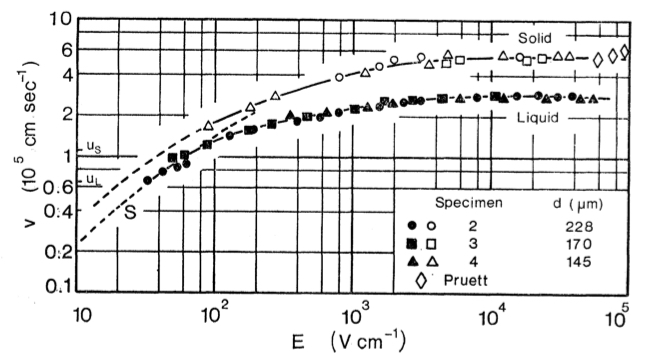
\includegraphics[angle=0.5, width=0.8\textwidth]{DriftVelocity}
\caption{Drift velocity for solid and liquid xenon}
\label{fig:drift_velocity}
\end{figure}
In addition to absorbing VUV photons impurities can attach to drifting electrons.






Page 257 in Aprile book